%****************************************************************************%
%* DIET Programmer's Guide                                                  *%
%*                                                                          *%
%*  Author(s):                                                              *%
%*    - Philippe COMBES (Philippe.Combes@ens-lyon.fr)                       *%
%*                                                                          *%
%* $LICENSE$                                                                *%
%****************************************************************************%
%* $Id$
%* $Log$
%* Revision 1.16  2010/12/28 17:50:48  bdepardo
%* Added \xspace in \diet command.
%* Typos.
%*
%* Revision 1.15  2010/07/07 15:10:51  amuresan
%* Added Cloud entry for the UsersGuide and ProgrammersGuide.
%*
%* Revision 1.14  2009/08/28 15:20:13  ecaron
%* Add information to generate the DIET tarball
%*
%* Revision 1.13  2008/04/07 22:26:26  ecaron
%* Updated files to pdflatex compilation
%*
%* Revision 1.12  2007/11/22 21:07:02  mimbert
%* use latex package fancyhdr instead of fancyheadings which seems deprecated in some recent latex distributions
%*
%* Revision 1.11  2007/04/17 13:34:52  ycaniou
%* Error in debug.tex header
%* Removes some warnings during doc generation
%*
%* Revision 1.10  2007/02/16 10:27:35  ycaniou
%* Beginning of a chapter on the Diet debugging (here, valgrind).
%*
%* Revision 1.9  2006/11/16 14:09:19  eboix
%* - Programmers guide converted from autotools to cmake.
%* - cmake summary deported to Cmake sub-dir.   --- Injay2461
%*
%* Revision 1.8  2006/06/30 21:20:37  eboix
%*   Cmake and dart related modifications:
%*    - [c]cmake's ambiguous option DIET_MAINTAINER_MODE removed. Building the
%*      documentation is now only controled by DIET_BUILD_DOCUMENTATION (and
%*      user's, developpers and doxygen docs are handled together). In order
%*      to use the Maintainer build type add -DCMAKE_BUILD_TYPE:STRING=Maintainer
%*      as [c]cmake option.
%*    - Created Cmake/Dart subdir as placeholder for Dart related utilities.
%*    - Cmake/DashBoardScript.cmake renamed to Cmake/Dart/DashBoardScript.cmake
%*                                                                 --- Injay2461
%*
%* Revision 1.7  2006/01/25 17:26:04  pfrauenk
%* CoRI : Some useful information about CoRI now available
%*
%* Revision 1.6  2005/08/08 08:26:57  ycaniou
%* Fixed remaining reference to ../UserManual/fig/logo in ProgrammersGuide.tex to ./fig/logo
%* Addition of a cp of the ../UserManual/fig/logo in the makefile: now it compiles
%* Addition of a batch section (also contains general remarks which have to be dispatched if pertinent). Not complete!
%*
%* Revision 1.4  2004/01/09 15:26:53  cpera
%* Add Annexe on Autotools.
%*
%* Revision 1.3  2003/12/15 00:13:53  ecaron
%* New structure for the first sheet
%*
%* Revision 1.2  2003/09/17 14:41:28  pcombes
%* Split the .tex according to its chapters.
%*
%* Revision 1.1  2003/09/09 12:42:44  pcombes
%* Reorganization of doc: include CS in a programmer's guide.
%****************************************************************************%

\documentclass[11pt,a4paper]{report}
\makeatletter
%\makeatother
\usepackage{fancyhdr}
%\usepackage[french]{babel}
%\usepackage[latin1]{inputenc}
\usepackage{multicol}
\usepackage{verbatim}
\usepackage{xspace}
\usepackage[headings]{fullpage}
\usepackage{url}
\usepackage[pdftex]{graphicx}
\graphicspath{{../UM/fig}}

\newsavebox{\logobox}
\sbox{\logobox}{
\includegraphics[scale=0.3]{fig/logo_DIET}}
\newcommand{\logo}{\usebox{\logobox}}

%%%%
\renewcommand{\title}{DIET Programmer's Guide}
%%%%

\pagestyle{fancyplain}
\lhead[\fancyplain{\title}{\title}]
      {\fancyplain{\title}{\title}}
\chead{}
\rhead[\fancyplain{\logo}{\logo}]{\fancyplain{\logo}{\logo}}

\lfoot[\fancyplain{INRIA}{INRIA}]{\fancyplain{INRIA}{INRIA}}
\cfoot[\fancyplain{}{}]{\fancyplain{}{}}
\rfoot[\fancyplain{Page~\thepage}{Page~\thepage}]
      {\fancyplain{Page~\thepage}{Page~\thepage}}


\newcommand{\fixme}[1]{\fbox{\textsl{{\bf FIXME: }#1}}}
\newcommand{\CMakeLists}{\textsf{CmakeLists.txt}\xspace}
\newcommand{\cmake}{\texttt{cmake}\xspace}
\newcommand{\diet}{\textsc{Diet}\xspace}

\begin{document}

%%%%
% First sheet
%%%%

\thispagestyle{empty}
\vspace*{3cm}
\vspace*{3cm}

\begin{center}

\includegraphics[scale=.5]{fig/logo_DIET}\\[2ex]
\textbf{\Huge PROGRAMMER'S GUIDE\\[2ex]}
\end{center}

\vfill


\noindent
\small{
\begin{tabular}{ll}
  \textbf{VERSION}  & 1.0\\
  \textbf{DATE}     & December 2003\\
  \textbf{PROJECT MANAGER}  & Fr\'ed\'eric \textsc{Desprez}.\\
  \textbf{EDITORIAL STAFF}  & Eddy \textsc{Caron} and Philippe ~\textsc{Combes}.\\
  \textbf{AUTHORS STAFF}    & 
\begin{minipage}[t]{12cm}
  Eddy \textsc{Caron}, Philippe ~\textsc{Combes}, Sylvain \textsc{Dahan}, Bruno \textsc{Delfabro}, Christophe \textsc{Pera}, Peter \textsc{Frauenkron} and Jean-Yves \textsc{L'Excellent}.
\end{minipage} \\
  \textbf{Copyright}& INRIA
\end{tabular}\\
}

\newpage
\thispagestyle{empty}
\ 

%%%%
% End of first sheet
%%%%

\newpage
\tableofcontents


\sloppy

%
% Introduction
%
\newpage
\addcontentsline{toc}{chapter}{Introduction}
\chapter*{Introduction}

This documents aims at giving to the new programmers of DIET a global
view of the software and it source code, so that they can quickly (and
cleanly) change it to fix bugs or to add new features.

The first chapter is dedicated to the installation of DIET as a
developer, to the use of CVS and the autotools.  The second chapter
describes the source tree, the roles of the various subdirectories and
some explanations about some very sensitive parts of the code (choices
for implementation, etc.)  In the last chapter, you will find the DIET
coding standards, in which we have collected a few guidelines to
follow when adding new source code or modifying the existing code.


%
% Getting started
%
\chapter{Getting started}
\label{ch:start}
%**
%*  @file  start.tex
%*  @brief   DIET Programmer's Guide - chapter one 
%*  @author  Philippe Combes (Philippe.Combes@ens-lyon.fr)
%*  @section Licence 
%*    |LICENSE|


\section{Using CVS}

There are two ways to get the source code for developers. DIET is
published under two forms of archive, and one of them contains all
files that are necessary to program in DIET: it is the maintainer mode
archive. But the most current way of getting the source files is to
use the CVS.

Here are the CVS environment variables to set (of course, the
programmer needs an account on the GRAAL server so far):
\begin{description}
\item{\sf CVSROOT} \textsf{ = :ext:graal.ens-lyon.fr:/home/CVS}
\item{\sf CVSUMASK} \textsf{ = 000}
\item{\sf CVS\_RSH} \textsf{ = ssh}
\item{\sf CVSEDITOR [optional]} your favorite editor.
\end{description}

Once all these variables are set, just execute\\
\centerline{\sf cvs checkout GRAAL/devel/diet}\\


As many developers work on DIET simultaneously, it is important to
commit files only when it is proved that it will not hinder the other
developers in their own work. The consensual use of simultaneous
developments is to perform an update of each file just before editing
it, then merge with the changes committed in-between and test the
local version to make sure that basic functionnalities are not
buggy. Commit the local version at last.

Deep changes should be preceeded by a discussion on the mailing list
\url{diet-dev@ens-lyon.fr} with all DIET developers.

On each commit, a log message is required. It is important that this
log message is clear enough for other developers to understand the
outlines of the changes, but it should remain concise. Try not to
exceed two 80 character-lines.  Indeed, the log messages are dumped
into the files headers.


\section{Bootstrapping}

The compilation of DIET is managed by Makefiles generated and
configured with \cmake.
\cmake generates a Makefile in each directory where there is a
\CMakeLists\ file.

If you have to add a file, or if you have to modify the compilation
dependence of an existing file in DIET, then you will have to modify a
\CMakeLists. 

\section{Configuring and compiling as a programmer}

Among the numerous options provided by the top \CMakeLists\ a
programmer should set the \verb+CMAKE_BUILD_TYPE+ to \verb+Maintainer+.
When doing so the compilers and linkers go paranoid and try to report
about most of the warning they are aware of.
Since the warning flags are compiler dependent this Maintainer build mode
is alas only available for GCC.

Here is the example of my source tree, got from the CVS server:
\begin{verbatim}
~ > cvs checkout GRAAL/devel/diet
~ > cd GRAAL/devel/diet
~ > mkdir Build ; cd Build
~ > cmake -DCMAKE_BUILD_TYPE:STRING=Maintainer <options> ..
...
\end{verbatim}

Finally, it is also strongly recommended to test your modifications
with a whole platform before submitting them.
A script \texttt{local\_platform} is given with the distribution
(in \textsf{bin/scripts}), which launches
\begin{itemize}
\item a mini LDAP base with the services \textsf{base/mult},
  \textsf{base/plus}, and \textsf{dgemm}, with the output of the FAST
  bencher that Martin made on his machine (but who cares right values
  for tests ?) ;
\item and four NWS entities: the three mandatory ones,
  \texttt{nws\_nameserver}, \texttt{nws\_memory} and
  \texttt{nws\_forecaster}, and one sensor for the local machine,
  \texttt{nws\_sensor} ; their ports are the ones used in the default
  configuration files of DIET.
\end{itemize}
So, as it is quite easy to launch a local platform, please do not
hesitate configuring DIET with FAST.

\section{Documentation}
\label{section:compiling-documentation}

Documentation is in \verb+CVS_DIET_HOME/doc+. It includes the LaTeX-based 
user's guide, the developer's guide and the doxygenated documentation.
Compilation of the documentation is very sensitive to the version of your
\LaTeX\ compiler and it also relies on many sub-dependencies
  (e.g. \verb+doxygen+ or \verb+fig2dev+)

\begin{itemize}
\item
  \verb+cd CVS_DIET_HOME/doc+
\item
  \verb+mkdir build+
\item
  \verb+cd build+
\item
  \verb+ccmake ..+ to enter the GUI
  \begin{itemize}
  \item press \verb+c+ (equivalent of bootstrap.sh of the autotools)
  \item toggle the desired options 
  \item specify the \verb+CMAKE_INSTALL_PREFIX+ parameter (if you wish
     to install in a directory different from \verb+/usr/local+,
  \item press \verb+c+ again, for checking required dependencies
  \item check all the parameters preceded with the * (star) character
     whose value was automatically retrieved by \verb+cmake+.
  \item provide the required information i.e. fill in the proper values
     for all parameters whose value is terminated by NOT-FOUND
  \item iterate the above process of parameter checking, toggle/specification
     and configuration until all configuration information is satisfied
  \item press \verb+g+ to generate the makefile
  \item press \verb+q+ to exit ccmake
  \end{itemize}
\item
  \verb+make+ in order to classically launch the compilation process
\item
  \verb+make install+ when installation is required
\end{itemize}


\section{Before altering DIET ...}

Once your environment has been set up, you are almost ready to add
your modifications in DIET. But, unless you are very well informed
about the way DIET is structured, please respect the following steps:
\begin{enumerate}
\item Decide which DIET entities are concerned by your changes.
\item ( For Eddy, are my changes \underline{\textbf{really}} useful ? )
\item Read carefully the paragraphs in chapter \ref{ch:tree} about the
  directory that deal with this entity (even if reading the chapter in
  a whole can only be a good thing ...).
\item Read \underline{\textbf{carefully}} the Coding Standards in
  chapter \ref{ch:CS}.
\item Include your modifications in the compilation chain (you may
  have nothing to do if you do not create any file, except your
  changes modify the dependencies)
\end{enumerate}


\section{Adding a file or a directory in the compilation chain}

%\fixme{Christophe - please check up and complete this part}\\

Understanding the conception of a \CMakeLists\ in DIET is quite
straightfoward.
Basically, we have to build two libraries (\textsf{DIET\_client}
and \textsf{DIET\_SeD}) and one binary executable (\textsf{dietAgent})
using great amount of common source code.

\subsection{Adding a file in a ``terminal'' directory}

A ``terminal'' directory is a directory where a library or an
executable is generated.\\

Let us take the example of the generation of the executable
\textsf{dietAgent}.
It is defined in the \texttt{src/agent/CMakeLists.txt}
with the following \cmake instructions:
\begin{verbatim}
ADD_EXECUTABLE( dietAgent dietAgent.cc )
TARGET_LINK_LIBRARIES( dietAgent AgentCommon)
\end{verbatim}

For the \textsf{DIET\_SeD} library, for instance, it would be:
\begin{verbatim}
SET( DIET_SeD_SOURCES
  DIET_server.cc
  DataMgrImpl.cc
  SeDImpl.cc
)
ADD_LIBRARY( DIET_SeD ${DIET_SeD_SOURCES} )
TARGET_LINK_LIBRARIES( DIET_SeD
  CorbaCommon
  IDLAgent IDLCommon
  UtilsCommon UtilsNodes UtilsSeDClt UtilsVector
  ${OMNIORB4_LIBRARIES}
)
\end{verbatim}

Thus, adding a \texttt{.cc} file in a ``terminal'' directory implies
only adding its name in the \texttt{*\_SOURCES} variable.

\subsection{Adding a file in a ``non-terminal'' directory}

In a ``non-terminal'' directory, we have to generate temporary
libraries that will be included in the final libraries
or executables. Of course it is possible to group all files of the
directory in a big library, but this would make the final libraries
and executables much bigger than necessary, since they would include
dead code (code that they would never use).
This is why we decided to group the files of each directory into
different libraries, depending on the ``destinations''
of the modules
\footnote{A module consists of a \textsf{.h} or
\textsf{.hh} and its associated \textsf{.c} or \textsf{.cc}.
For instance, the header and the implementation of a class.},
i.e.~depending on the final binaries that use them.
Please refer to the dependency table \ref{t:dep}, which every
DIET programmer is asked to maintain whereas he alters the repartition
of these libraries, because of new files or modifications that
change the dependencies.  \\

\noindent
To add a new module in a non-terminal directory,
\begin{enumerate}
\item Add its line in the table \ref{t:dep} (in the section of its
  directory), and put an 'x' in each column where it is used.
\item Then you can find to which temporary library you must add it:
  the library that matches the same combination of 'x' in the table,
  or if none, a new one.
\item Add the \textsf{.cc} file in the corresponding
  \texttt{*\_SOURCES} variable of the \CMakeLists\ in the directory.
\end{enumerate}

\begin{table}[h]
 \footnotesize
 \centering
 \fixme{Bruno - Pease add your files for data persistency ...}
 \begin{tabular}[c]{|l|c|c|c|l|}
  \hline
  Modules  &
  \begin{minipage}[c]{1.65cm}
   \centering used in\\ \texttt{dietAgent}
  \end{minipage}                  &
  \begin{minipage}[c]{1.65cm}
   \centering used in\\ \texttt{DIET\_SeD}
  \end{minipage}                  &
  \begin{minipage}[c]{1.65cm}
   \centering used in\\% \hspace*{-5pt}
   \texttt{DIET\_client}
  \end{minipage}                  &
  \textsf{.la} library to add to\\[5pt]
  \hline

  % AGENT
  \multicolumn{1}{|l}{\textsf{src/agent}:} &
  \multicolumn{4}{l|}{\texttt{dietAgent}}\\[5pt]

  \textit{all files}              & x &   &   & \emph{none}\\[5pt]
  \hline

  % CLIENT
  \multicolumn{1}{|l}{\textsf{src/client}:} &
  \multicolumn{4}{l|}{\texttt{libDIET\_client.[a|so]}}\\[5pt]

  \textit{all files}              &   &   & x & \emph{none}\\[5pt]
  \hline

  % CORBA
  \multicolumn{1}{|l}{\textsf{src/CORBA}:} &
  \multicolumn{4}{l|}{\texttt{libCorbaCommon.la}}\\[5pt]

  \texttt{marshalling}            & x & x & x & \texttt{libCorbaCommon.la}\\
  \texttt{ORBMgr}                 & x & x & x & \texttt{libCorbaCommon.la}\\[5pt]
  \hline

  % CORBA/idl
  \multicolumn{1}{|l}{\textsf{src/CORBA/IDL}:} &
  \multicolumn{4}{l|}{\texttt{libIDLCommon.la libIDLAgent.la
                              libIDLLA.la libIDLMA.la}}\\[5pt]

  \texttt{Agent[Dyn]SK}           & x & x &   & \texttt{libIDLAgent.la}\\
  \texttt{LocalAgent[Dyn]SK}      & x &   &   & \texttt{libIDLLA.la}\\
  \texttt{MasterAgent[Dyn]SK}     & x &   & x & \texttt{libIDLMA.la}\\
  \texttt{Callback[Dyn]SK}        & x & x & x & \texttt{libIDLCommon.la}\\
  \texttt{SeD[Dyn]SK}             & x & x & x & \texttt{libIDLCommon.la}\\
  \texttt{common\_types[Dyn]SK}   & x & x & x & \texttt{libIDLCommon.la}\\
  \texttt{response[Dyn]SK}        & x & x & x & \texttt{libIDLCommon.la}\\
  \texttt{DataMgr[Dyn]SK}        & x & x & x & \texttt{libIDLAgent.la}\\
  \texttt{LocMgr[Dyn]SK}        & x & x & x & \texttt{libIDLAgent.la}\\[5pt]
  \hline

  % SED

  \multicolumn{1}{|l}{\textsf{src/SeD}:} &
  \multicolumn{4}{l|}{\texttt{libDIET\_SeD.[a|so]}}\\[5pt]

  \textit{all files}              &   & x &   & \emph{none}\\[5pt]
  \hline

  % UTILS

  \multicolumn{1}{|l}{\textsf{src/utils}:} &
  \multicolumn{4}{l|}{\texttt{libUtilsCommon.la
                             libUtilsSeDClt.la  libUtilsNodes.la}}\\[5pt]

  \texttt{Counter}                & x & x &   & \texttt{libUtilsNodes.la}\\
  \texttt{Cori*}                  & x & x &   & \texttt{libUtilsNodes.la}\\
  \texttt{CORIMgr}                & x & x &   & \texttt{libUtilsNodes.la}\\
  \texttt{debug}                  & x & x & x & \texttt{libUtilsCommon.la}\\
  \texttt{DIET\_data}             & x & x & x & \texttt{libUtilsCommon.la}\\
  \texttt{DIET\_mutex}            &   & x & x & \texttt{libUtilsSeDClt.la}\\
  \texttt{ms\_function}           & x & x & x & \texttt{libUtilsCommon.la}\\
  \texttt{Parsers}                & x & x & x & \texttt{libUtilsCommon.la}\\
  \texttt{ServiceTable}           & x & x &   & \texttt{libUtilsNodes.la}\\
  \texttt{statistics}             & x & x & x & \texttt{libUtilsCommon.la}\\[5pt]
  \hline


 \end{tabular}
 \caption{Dependencies of the final binaries from the temporary
 libraries}
 \label{t:dep}
\end{table}


\noindent
\fbox{\textbf{NB}} The particular case of the sub-directory
\textsf{IDL} will be discussed in section \ref{s:IDL}. Indeed, it
cannot be processed as the other ones, since the \textsf{.idl} files
are the true source files. The \textsf{.cc} and \textsf{.hh} files are
``built sources'' generated from the \textsf{.idl}.



\subsection{Adding a directory}

We will discuss here the criteria that makes the creation of a new
directory sensible. We will just mention, as exposed in the
\textit{Coding Standards} (chapter \ref{ch:CS}), that such changes
should be discussed on the developers mailing list,
\url{diet-dev@ens-lyon.fr}.  \\ We will not discuss neither the way to
add the directory in the CVS repository, since this has nothing to do
here.

Once it has been decided to add a new directory, and once its own
\CMakeLists\ is written, then it has to be reported
in the \CMakeLists\ of its parent directory.
It should be added with a \texttt{ADD\_SUBDIRECTORY} command.



%
% The source tree
%
\chapter{The source code tree}
\label{ch:tree}
%**
%*  @file  source_tree.tex
%*  @brief  DIET Programmer' guide - chapter two
%*  @author  Philippe Combes (Philippe.Combes@ens-lyon.fr)
%*  @section Licence 
%*    |LICENCE|


There are two main source directories, \textsf{include} and \textsf{src}, and
the \textsf{doc} directory.


\section{\textsf{doc}}
\label{s:doc}

This directory contains documentations that are to be maintained up-to-date,
even in CVS, (\emph{ie} \textbf{not only for releases !}):

  \begin{itemize}
  \item \textsf{doc/UsersManual} contains the \textit{User's Manual}. 
     Its output file is \texttt{DIET\_UsersManual.ps}, which is intalled in
     \texttt{$<$install\_dir$>$/doc}.
  \item \textsf{doc/ProgrammersGuide} holds the \textit{Programmer's Guide}.
     Its output file is \texttt{DIET\_ProgrammersGuide.ps}, which is intalled
     in \texttt{$<$install\_dir$>$/doc}, \textbf{if} DIET has been configured
     in maintainer mode.
  \item \textsf{doc/Tutorial} holds a tutorial, which is only available
     in the CVS version, since the distribution of this tutorial is apart
     from the distribution of the source code.
  \item \textsf{doc/ExternalExample} contains a minimal set of files
     that enable to illustate how a DIET user can compile and link
     against an installation of DIET.
     This can be done both with \verb+make+ and \verb+cmake+.
     Note that the purpose of this directory is not to demonstrate
     DIET features.
     Nevertheless, the very simple DIET client/server example is effective
     DIET code.
  \end{itemize}

  The compilation of this documentation may require too recent versions of
  \LaTeX and of various converters for the figures.
  This is why, the output \textsf{.ps} files are included in the distributions.

  \section{\textsf{include}}
  \label{s:include}

  This directory contains all the files necessary for the DIET user to program his
  application. Almost all these files are headers which are copied into the
  \textsf{$<$install\_dir$>$/include} directory, because they describe the
  complete API of DIET, for the client side as well as for the server side.

  Nevertheless, there is also a \texttt{Makefile.inc.in} which will be configured
  into a \texttt{Makefile.inc}.
  The latter is to be included by the \texttt{Makefile} of the
  DIET user, to set all options and variables necessary for compiling and
  linking with the DIET libraries.
  It may be noticed that some variables are affected with
  \texttt{?=} ; it is because the \texttt{Makefile.inc} is also included by the
  DIET examples, which need to define a different prefix as long as the
  \texttt{make install} has not been invoked.



  \subsubsection{\tt DIET\_data.h}

  The first file to be included. It describes all types and data structures (and
      the associated functions and macros) that are common to the interfaces of the
  client and the server: \verb+diet_arg_t+, \verb+diet_profile_t+, \verb+*_set+
  and \verb+*_get+ functions, \verb+diet_free_data+, etc.

  Please note that the \verb+*_get+ functions are actually macros, which allows
  the user not to care about the type of the data. But the compilation of a
  program that uses such macros could trigger a warning about ``strict aliasing''.
  This is the case for the distributed examples, when compiled with
\textsf{gcc-3.3} or later (see section \ref{s:examples})


  \subsubsection{{\tt DIET\_client.h} and {\tt DIET\_grpc.h}}

  The specific part of the client interface is described in these two files.
  \textsf{DIET\_client.h} includes \textsf{DIET\_grpc.h}, which includes itself
  \textsf{DIET\_data.h}.
  The first file is the DIET specific API, adpated and optimized for the data
  structures of DIET. The second file consists of the GridRPC API, even if some of
  the functions are not fully implemented (for more details, please read the
      numerous comments of the file itself).


  \subsubsection{\tt DIET\_server.h}

  This file contains the specific part of the server API.
  It offers functions and macros to manipulate the description of the service
  profiles (\verb+diet_profile_desc_t+), and store them into the service table of
  the server (\verb+diet_*service_table*+). Everything that concerns the problem
  profiles (how to extract their arguments, set their OUT arguments, etc.) is
  described in \texttt{DIET\_data.h}.


  There is also the complete API to the \texttt{diet\_convertor\_t} structures.
  Their usage are (or should be) explained in the \textit{User's Manual}, and the
  way they are applied is fully documented in section \ref{s:CORBA}, since the
  conversions are performed by functions of the file \texttt{marshalling.cc}.

  \subsubsection{\tt DIET\_mutex.h}

  This is intented to be a portable API to the various thread libraries, a bit
  like the \textsf{omnithread} library. But the \textsf{omnithread} library is a
  portable API for all thread systems (pthreads for Linux, but also the official
      thread libraries of other platforms), and {\tt DIET\_mutex.h} should only unify
  the APIs of different ORBs, since they all offer a portable thread library.
  Thus, as well as an application using \textsf{omniORB} should use the
  \textsf{omnithread} library if it has to deal with threads, an application using
  DIET will have to use the DIET thread library.

  It is not documented yet in the \textit{User's Manual} because it is really not
  ready to be distributed. Currently it deals only with mutexes, and waits for a
  complete development...



  \section{\textsf{src/agent}}
  \label{s:agent}

  \subsection{The hierarchy of agents}

  This section deals with the inheritance of the C++ agent classes and the way an
  agent refers to its children. The inheritance hierarchy of the CORBA objects
  will be treated in section \ref{s:IDL}.
  \\

  The hierarchy of the C++ classes that implement the CORBA interfaces is mapped
  onto the hierarchy of theses interfaces, \emph{i.e.} \textsf{LocalAgentImpl} and
  \textsf{MasterAgentImpl} both inherit from \textsf{AgentImpl}. Thus, Most of the
  public function members of each class are implementations of IDL methods.

  In \textsf{AgentImpl}, \texttt{getName} is especially added for the data
  persistency architecture.

  In all classes, it has been added a \texttt{run} method that makes the
  \texttt{main} function (in \texttt{dietAgent.cc}) launch the agent. This method
  has two parts: the generic part is declared and implemented in the
  \textsf{AgentImpl} class, and the parts specific to the LA or the MA are
  declared in these classes. As these declarations overwrite the \texttt{run}
  method of \textsf{AgentImpl}, their implementations call explicitly the parent
  method.

  The protected part of the \textsf{AgentImpl} is inherited by both the
  \textsf{LocalAgentImpl} and \textsf{MasterAgentImpl}, and it groups the common
  members (the \textsf{ServiceTable}, the lists of children and requests, etc.) as
  well as the common parts of the code: the way to forward a request, to aggregate
  the responses, and some methods useful in all these jobs.
  \\

  The architecture of agents is handled with a pointer to the parent
  (\verb+Agent_var parent;+) in \textsf{LocalAgentImpl}, and two vectors of children
  in \textsf{AgentImpl}, one for LAs and one for SeDs. These vectors of children are
  actually \textsf{ts\_vectors} of instances of \textsf{NodeDescription}. The
  latter has to store information such as the hostname, the child ID (since
      children are referred to with their indexes in the vectors) but above all the
  CORBA reference of the child (an \textsf{LA\_var} or an \textsf{SeD\_var}). That
  is why it has to be a template.


  \subsection{The requests}

  The requests are managed through a class that stores all informations
  about the requests, such as their ID, the responses returned by the SeD and LA
  and the scheduler to use for the request.

  A mechanism have been developed to manage the waiting of all the responses
  returned by the SeD and LA. The \texttt{waitResponses()} methods will block the
  current thread until a defined number of call of the \texttt{addResponse()}
  method have been made. Look at the doxygen documentation for more information.


  \subsection{The schedulers}

  When all the children of an agent have sent back their responses, the agent must
  aggregate and sort them into the one single response it will sent to its parent.
  This aggregation/sort is performed by the scheduler classes.

  The starting point of the development of these scheduler classes was a
  combination of two ideas:
  \begin{itemize}
  \item Some servers would never have FAST fully installed. Either because FAST or
  NWS does not support the hardware architecture, or because the services
  offered cannot be described in the FAST ``language'' accurately enough for a
  valid bench campaign or estimation, etc. The information that the servers can
  give to the scheduler are very heterogeneous, and the old DIET scheduler was
  dealing with only the FAST estimations.\\
  An other tool has been implemented, called CoRI, and will be used to get by 
  default the information and to get other types of information (total memory,...).
  At the moment it is not compiled/called by default. This will be change when
  it is matured. See section \ref{subsection:performance} for more information.
  \item For research aspects on the platform, it would be very interesting to
  have pluggable schedulers. As the old scheduler was integrated to the agent,
  the first step towards pluggable schedulers was building classes responsible
  for the scheduling.\\
\fixme{plugin is made by alan su!}
  \end{itemize}

  The heterogeneity of the information given by the servers is due to the fact
  that all servers cannot provide the same level of accuracy about the evaluation
  of a request. We have thought of 4 different levels of accuracy, and one
  \textsf{Scheduler} class deals with one and only one level.
  \begin{enumerate}
  \item No information at all: such servers are not sorted but placed randomly.
  \item Last solve time: such server are sorted according to the last solve time.
  \item Hardware information (disk space, RAM, CPU speed, etc.): not managed yet.
  \item Dynamic information (CPU load, free memory, given by NWS): such servers
  are sorted according to their weight, which is a polynom of these
  characteristics, including the data transfer time if available.
  \item Estimation of the computation time (performed by FAST): such servers
  are sorted according to the computation time estimated plus the data transfer
  time estimated.
  \end{enumerate}

  Actually, there are only four schedulers implemented, because nothing has been
  done yet for the servers to get static information (level 3).\\
  Actually, with the compiling option --enable-cori only scheduling with round
  robin (last solve time - level 2) and random scheduling (level 1) is possible.
  There are multiple reasons why no other scheduling is possible:
\begin{enumerate}
  \item The NWS scheduling is bogus: the weight for the memory is too
  heavy in comparison with the free CPU. Fixing is not so easy, so
  we deciding to test with several plugin schedulers their
  performance, before implementing a default scheduling.
  \item To avoid an increasing complexity of the context.
  \item To avoid a single server equipped with FAST will always be chosen by
  the agent.
  \item The plugin scheduler can be used now with all power, it will
  be possible to define a scheduler for each server. It is very easy to recreate the old 
fast scheduling by the plug-in.
  \end{enumerate}


  Once the schedulers have sorted every group of servers, the most difficult is
  still to do. How to combine the various information of the servers to get a
  whole sorted list ? Which parameters should we give priority to ? This is the
  role of the \textsf{GlobalScheduler} classes. They are schedulers of the
  schedulers. A \textsf{GlobalScheduler} has got a sorted list of schedulers
  (\texttt{SchedList schedulers}) to apply onto the lists of servers. This
  presents the drawback that the agent sorts by category of information before
  sorting the servers inner each category: it is not possible to mix the various
  categories yet. But it would be easy to implement schedulers that take into
  account all type of information, computing a weight as for NWS information. It
  is just not done, because our goal was to build a frame for developping new
  schedulers, and not to test various policies.

  The only \textsf{GlobalScheduler} available so far (\textsf{StdGS}) calls first
  the \textsf{FASTScheduler} onto the list, putting ahead the servers that could
  estimate the request, then the \textsf{NWSScheduler} (for NWS information), then
  the \textsf{RRScheduler} and finally the \textsf{RandScheduler} that add the
  servers randomly into the list.
  \\

  Several drawbacks can be noticed about such a structure of schedulers:
  \begin{itemize}
  \item It is not possible to mix the various categories of servers.
  \item The schedulers are not pluggable at all.
  \item A global scheduler must be associated to each request, so that every
  agent, at every level, will schedule it the same way. But if we let the
  servers decide, they will choose different schedulers ; so only the MA can
  choose it, and as soon as the request arrives from the client ! Then it
  forwards the scheduler (its serialzed form actually) with the request, before
  it gets any information about the servers.
  \item The classes \textsf{GlobalScheduler} and \textsf{Scheduler} are actually
  virtual (because of their respective \texttt{sort} method). Thus, they
  constitue an interface that every new scheduler (global or not) should
  implements, and some maintainers may find this interface a bit too rigid, but
  it is the only way I found to get the scheduler out of the agent.
  \end{itemize}

  Despite these drawbacks, it is now much easier to change the scheduler used in
  the agent. But there is still a lot to do to reach the pluggable schedulers, if
  ever it is possible.

  \subsection{Performance prediction}\label{subsection:performance}
  CoRI is now implemented to get more information about the SeD.
  It is called by the server's side and (in FAST mode) on the agent's side. 
  CoRI is a simple super layer that manages multiple sub modules. One module
  is Cori-Easy; another is FAST.

  \subsubsection{Using Cori}
  The programmer of DIET services will use the
  interface proposed in the SeD interface file, \textsf{DIET\_server.h}
  Using CoRI as programmer DIET, use directly the
  \textsf{CORIMgr.hh}
  The starting phase of cori can be described as follow:
   \begin{itemize}
  \item All desired collectors will be add by \texttt{add} 
  \item Launch the \texttt{startCollectors} to initialising some collectors
    (i.e FAST) on startup of the server
  \item using the \textsf{call\_cori\_mgr} function on 
    demand to get a value in the estVector.
  \end{itemize}
  
  Additional to the tags that the programmer of DIET
  service can use, the DIET programmer can use 
  the tag EST\_COMMTIME for FAST. It is agent side only. 

  \subsubsection{CoRI-Easy}
  Cori-Easy is based on basic system calls. There are different
   levels to obtain this information: 
  The best way is the most portable way: The standard C library. For examples the
  functions \texttt{get\_Write\_Speed} and \texttt{get\_Read\_Speed} are written in pure C.
  OmniORB is used by DIET and it needs the GNU Library C standard, 
  so this library is the next level.
  The third level is the POSIX standard. Remark: even if Red Hat 
  say they follow the POSIX standard, this doesn't mean that you have to include the same file
  to get the function of the POSIX standard (for example \texttt{getPID()}). 
  It means you can never be sure to have the function!
  The fourth level is the distribution of the operating system, 
  but even here you have to take care(new version-old version conflicts). 
  System calls are very fragile, point of view accessibility 
  (they are not always present or you have to be root to execute them)
  , point of view functionality of the function (``top -n 1'' 
  in Linux is different to ``top -n 1'' in Mac).
  and point of view presentation of the output data (is it sure that 
  he will print it always on the second line?).

  Very important to avoid problems in the compilation is the use of 
   \texttt{\#ifdef HAVE\_nameFunction}.  
  The calls to cori-easy are in reality a set of tests. If the first function doesn't work,
  the next one is tested. In this way we avoid to write for each 
  distribution a test to identify this distribution and we avoid to 
  have to find out the right function for this special distribution.

  \fixme{Problems with  the function \texttt{diet\_est\_cori}}
  \begin{itemize}
 \item called twice in the same tag for a scalar values, the second will erase the first
  \end{itemize} 

\subsubsection{Availability}
CoRI Easy will be used to initialize the vector by default. The problem is that even Cori-Easy is not always able to call a function that gives the correct value. That's why it is important to deliver the default value.
\fixme{set up a table with the default values} 
  \subsubsection{Extensibility}
  CoRI is supposed to be extensible, by adding a new API and a new tag
  of type \texttt{diet\_est\_collect\_tag\_t} in the
  CoRI class structure.
  The file \textsf{Cori\_Data\_Easy} is used as interface between
  CoRI and the Cori-Easy collector.
 \subsubsection{Examples  with the scheduler}
 See /home/CVS/tarballs/scheduler\_cori\_examples.tar.gz  on the graal server (perhaps bogus).
 \subsubsection{FAST as collector of CoRI}
 Fast will be launched on the server side only on demand of the plugin scheduler.
 FAST will be launched automatically on the MA and LA side.\\
 \fixme{launching only if need?}\\ Would it be interesting to be able to start fast on the MA side dynamicaly?\\
\fixme{FAST without CoRI}\\ 
In this case all possible fields of the vector will be filled (i.e. erase old values).

  \section{\textsf{src/client}}
  \label{s:client}

  This directory contains the implementation of both client APIs, the DIET API and
  the GridRPC API.

  The GridRPC is actually incompatible with the strictly defined types used in
  DIET, which avoid many run-time errors. That is why the \texttt{gridrpc\_call}
  functions is a bit modified, as it requires \texttt{diet\_arg\_t} arguments
  only.

  %\fixme{Christophe - the asynchronous part of the API}


  \subsection{synchronous call in DIET}
  Synchronous DIET call are based on \emph{twoway} CORBA call. CORBA manages synchronizing
  and memory. Main problems and architectures related to this kind of call concerns
  DIET types, modified memory management increasing performance and convertors (see section \ref{s:CORBA}).

  \subsection{asynchronous call in DIET}

  \subsubsection{Architecture}

  \emph{omniORB} is chosen because of its performance. But its implementation
  of standard CORBA specification is not full. For instance, \emph{AMI}
  (Asynchronous Message Interface) or sending object by value are not yet
  available. According to this lack of services, we must based asynchronous
  communication architecture on its avalaible services.
  Two basic CORBA mecanisms can allow this asynchronous architecture.
  First is using IDL key word \emph{oneway} which delegates \emph{thread} managing
  to \emph{POA} (Portable Object Adaptor) and stops immediatly after sending data parameters. This thread
  executes solver code and return explicitly results data to client.
  Secondth uses standard CORBA synchronous call.
  \emph{RPC} creates a thread, delegates algorythm executing to it and returns.
  Executed algorythm solves its problem and return results data to clients or stores
  it (waitting for client get it).

  Getting a result from an asynchronous call can be done by \emph{polling} or
  \emph{callback} mecanism.

  \begin{description}
  \item[\emph{Callback} mecanism] allows SeD process to bind client and send results data.
  During asynchronous call (solveAsync methode)to begin SeD solve, client
  add to send data its CORBA reference identifiing a local CORBA server
  waiting results and a request identifier.
  As soon as results are available, they are sent to client callback CORBA server
  with its request identifier by calling \emph{notifyRst} server's function.
  Data structures sent to SeD server or return to client callback server are like
  them of synchronous call. Currently, client callback server reference and request
  identifier are volatile.
  \item[\emph{Polling} mecanism] will use next DIET data persistency mecanism.
  Results data will be store locally or exported to a persistency service.
  They will be avalaible through DIET persistency API. This mecanism is under
  development as polling service. It will replace callback when presistence will
  by critical.
  \item[DIET release 1.0] provides only asynchronous with callback function. Its
  implementation is hidden by DIET and GridRPC API on client side. All asynchronous call
  and synchronized waiting results functions are \emph{thread-safe}.
  \end{description}

  \subsubsection{Coding}
  \paragraph{Callback}
  Callback 's module is part of DIET client library. It contains classes generated
  from \emph{callback.idl} file by CORBA idl compiler and CallbackImpl class
  which provides functions for waiting and managing results. It is a \emph{singleton}
  \emph{thread-safe} class.

  %\begin{figure}[h]
  %\begin{center}
  %\centering
  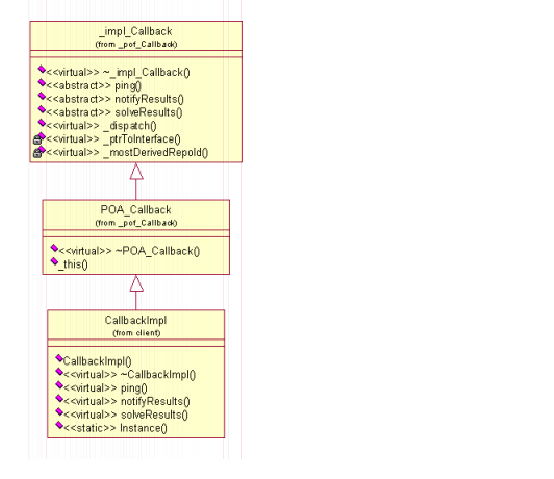
\includegraphics{./fig/CorbaClientClassDIagram}
  %\caption{UML Class diagram about Callback mecanism}
  %\label{fig:CorbaClientClassDIagram} 
  %\end{center}
  %\end{figure}

  Class constructor is private. It is accessed by a static class function
  \emph{CallbackImpl::instance} which returns a sole object instance. It
  creates object, initialises its class data and CORBA context, provides a
  client callback CORBA server on network.
  Client code must only give its CORBA reference when calling asynchronous
  function \emph{solveAsync}.s
  SeD server calls \emph{CORBA} \emph{solveResult} function with this
  reference to send results to client callback server.
  Combining  a call to \emph{diet\_initialise} and DIET file option
  \emph{useAsyncCall} automates client callback mecanism.
  A \emph{diet\_finalize} call unactivates callback server, destroys
  CallbackImpl object and Object Request Broker data.

  \paragraph{synchronizing data}
  Synchronising access on data is necessary because of:
  \begin{itemize}
  \item Threads can together retrieve results data.
  \item CORBA threads pool from client callback server read concurrently
  profil data structure.
  \item DIET API function \emph{diet\_wait*} stop caller thread until wait
  results data are arrived on client.
  \end{itemize}
  Classes from following UML diagram resume these drawbacks.

  %\begin{figure}[h]
  %\begin{center}
  %\centering
  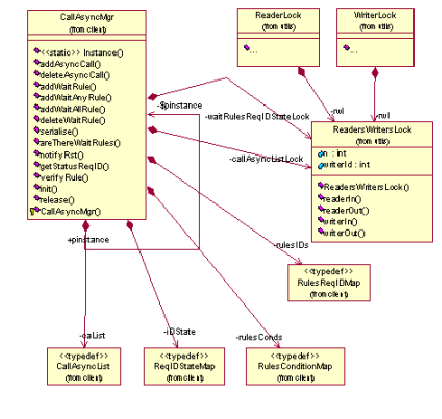
\includegraphics{./fig/CallBackSynchronisationClassDiagram2}
  %\caption{Diagramme UML class diagram about callbackImpl and GridRPC/DIET asynchronous functions}
  %\label{fig:CallBackSynchronisationClassDiagram2}
  %\end{center}
  %\end{figure}

  CallAsyncMgr manages synchronising mecanism on wait results. It is a \emph{thread-safe}
  singleton which locks access on share data and race condition code. A
  \emph{diet\_initialise}/\emph{diet\_finalise} call creates/destroys it. A
  Reader/Writer lock mecanism (exception-safe) manages syncronising between
  CORBA and DIET client threads.

  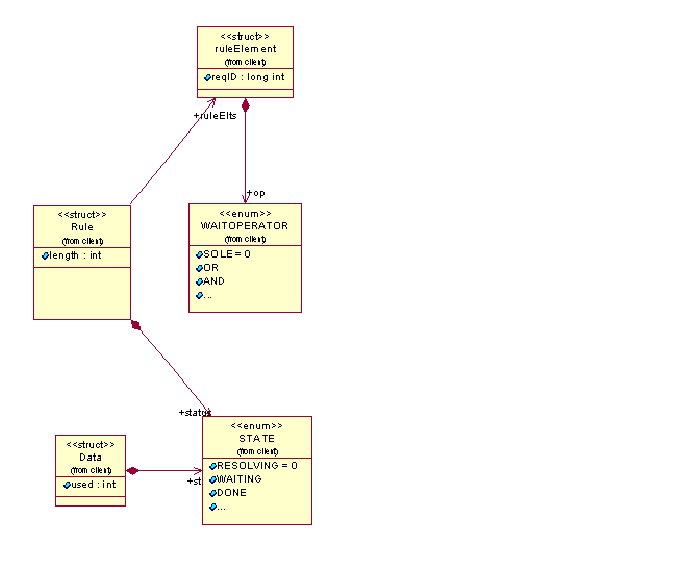
\includegraphics{./fig/WaitRulesClassDiagram}

  \emph{CallAsyncMgr} register/unregister asynchronous calls, their request
  identifiers and data by \emph{addAsyncCall}/ \emph{deleteAsynCall} methode.
  It stops client threads with addWait* methodes. These methodes have
  parameters which store conditions on retrieved results to unlock threads.
  A \emph{Rule} structure contains a set of three data (request identifier,logical operator, state).
  Two list of data pair (\emph{RulesConditionMap} and \emph{CallAsyncList}) map \emph{Rule} with a
  lock reference and request identifier with a DIET data
  profil. \emph{notifyRst} methode allows CORBA threads to announce results getting,
  update data in memory client space, unlock one or more waited threads.

  %\subsubsection{Synchronising and interworking}
  \paragraph{Synchronising and interworking}
  In following scenarios, an UML actor figures user client code with DIET/GridRPC API.

  \subparagraph{Asynchronous call on a SeD:}
  This first scenario shows a begining of an asynchronous solve.

  %\begin{figure}[h]
  \hspace{-0.9 in}
  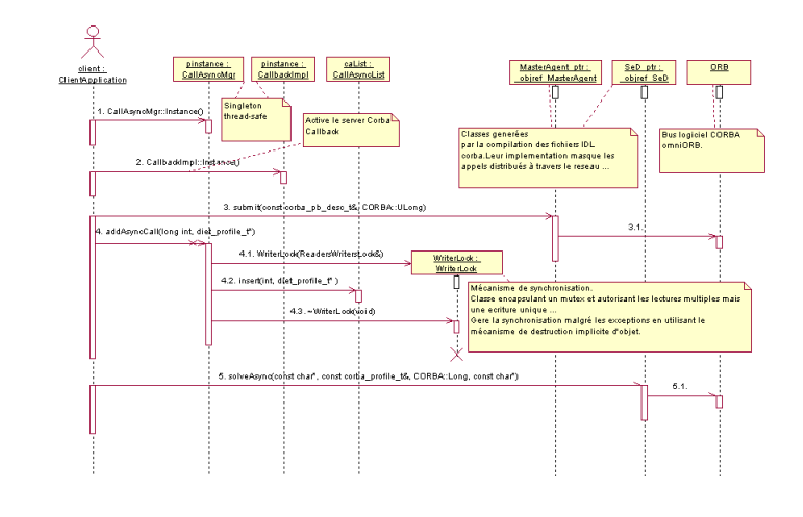
\includegraphics{./fig/CallAsyncSequenceDiagram}
  %\end{figure}

  After creating CallbackImpl and callAsyncMgrby a call to
  \emph{diet\_initialize}, client execute submit function specifying DIET
  problem. Then, \emph{addcallAsync} methode stores a sole request
  identifier and managed memory space and \emph{solveAsync} starts
  asynchronous solve.
  CallAsyncList is a C++ container \emph{list} from \emph{Standard Template Library}
  \emph{ORB} entity is a virtual object figuring CORBA services API like
  marshalling, network traffic and CORBA object binding.
  Client thread can wait for notify event about satisfied conditions or
  poll results states by frequently call to \emph{getStatusReqId} methode.

  \vspace{.9 in}

  \subparagraph{Thread Waiting for results and then continue:}
  Solve is started and client thread can wait for results.

  \hspace{-1 in}
  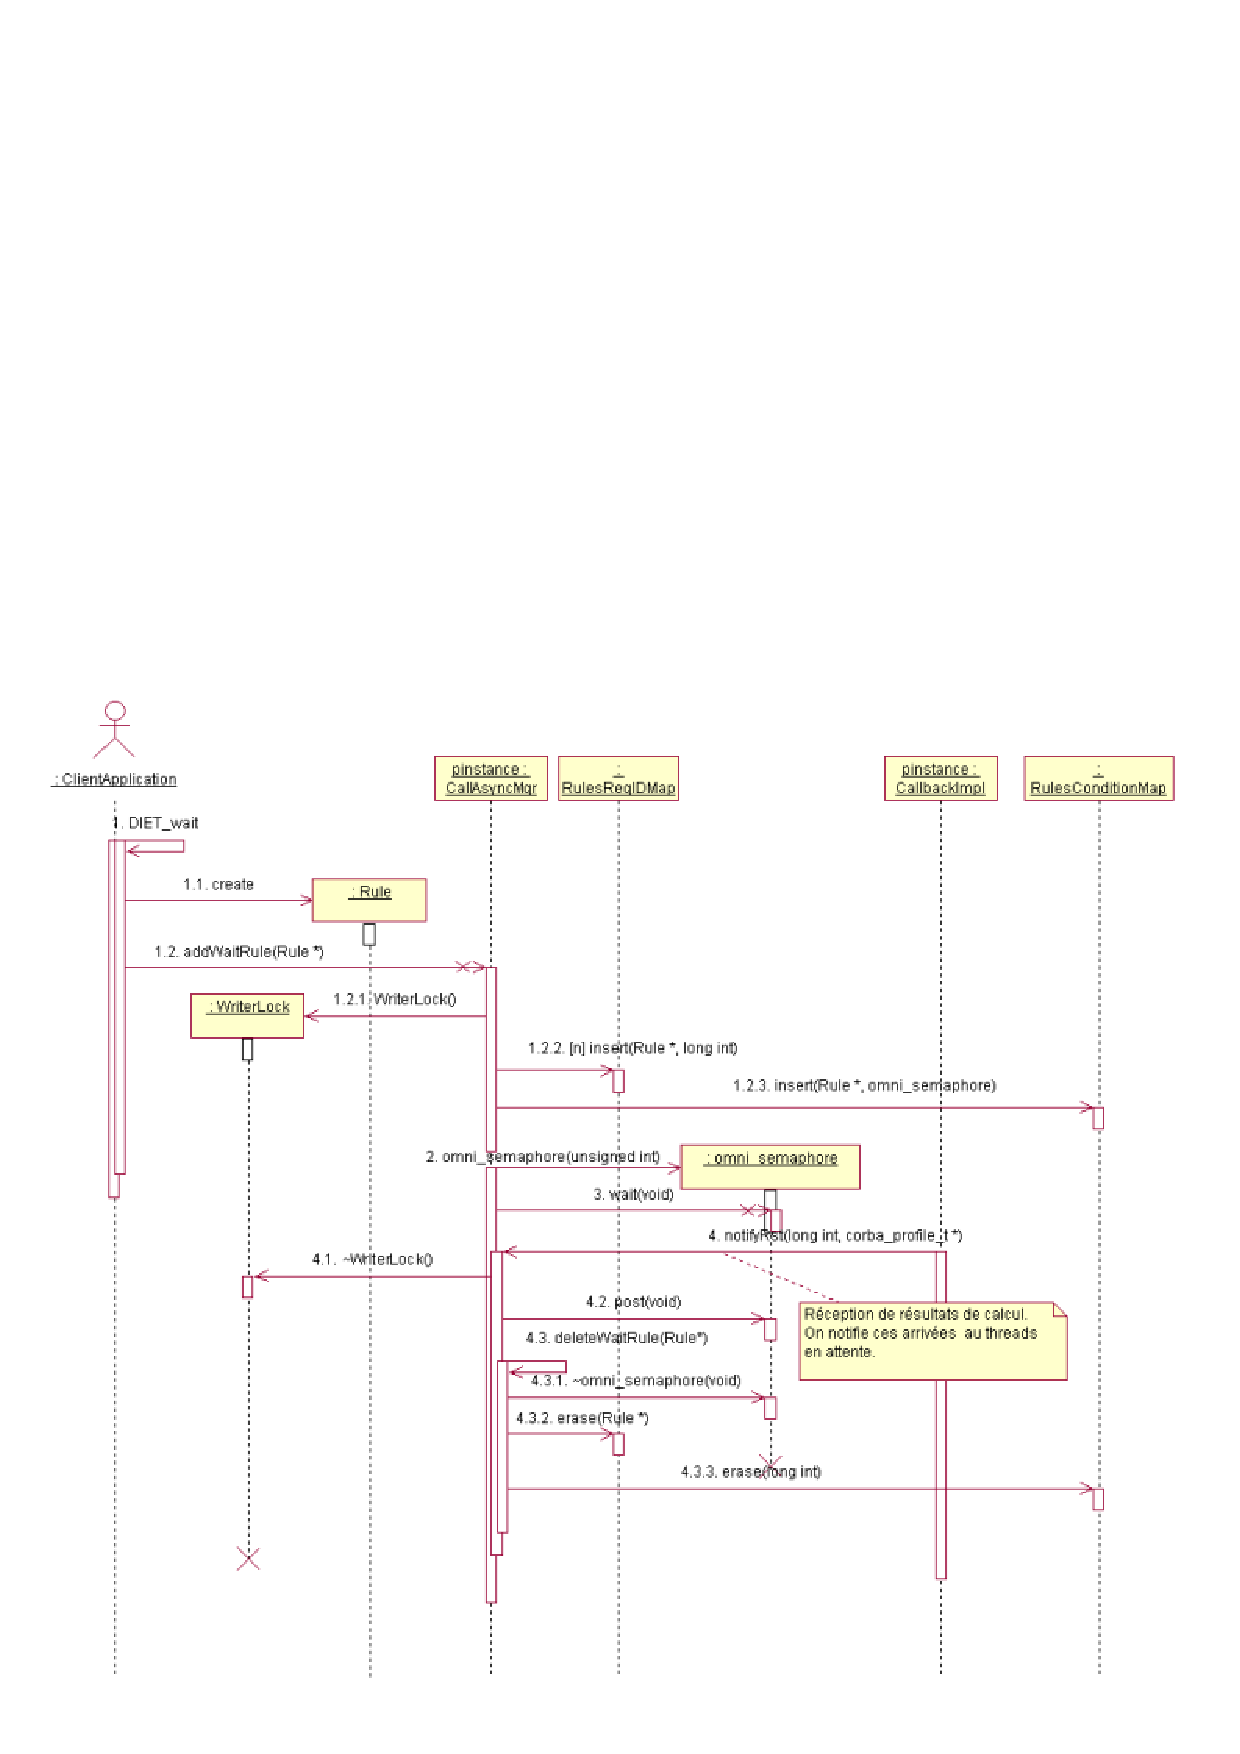
\includegraphics{./fig/CallAsyncWaitSequenceDiagram}

  Client code can use synchronising functions like \emph{diet\_wait*}
  in GridRPC/DIET API to wait for results. The following text describes
  this mecanism.

  After calculus starting, client creates a waiting Rule which specifies
  waiting conditions. Then it calls \emph{addWaitRule} methode which do :

  \begin{itemize}
  \item locks synvhronising mecanism.
  \item validates rule data (request identifier, etc).
  \item registers the rule.
  \item creates an \emph{omniORB}  semaphore, maps to the rule, registers it,
  unlocks synchonising mecanism (\emph{WriterLock}) and call its \emph{wait} methode.
  \item during call to \emph{notifyRst} methode by \emph{Callback} server
  (\emph{calbackImpl}), finds all rules whose conditions are verified
  and unlock their semaphores.
  \item frees memory linked to rule data and returns a \emph{STATE} enum
  which defines five state (RESOLVING, WAITING, DONE, CANCEL, ERROR). If
  a calculus is stopped during its executing process (with a call to deleteCallAsync for example),
  CANCEL is returned. If thread catches an error or an exception, ERROR is returned else DONE is returned.
  \end{itemize}


  \subparagraph{Getting results into callback server and notifying them to waiting threads :}
  This scenario figures notifying available results into client. It completes
  the previous algorythm about threads using client gridRPC API which is a
  part of DIET client library.

  \begin{center}
  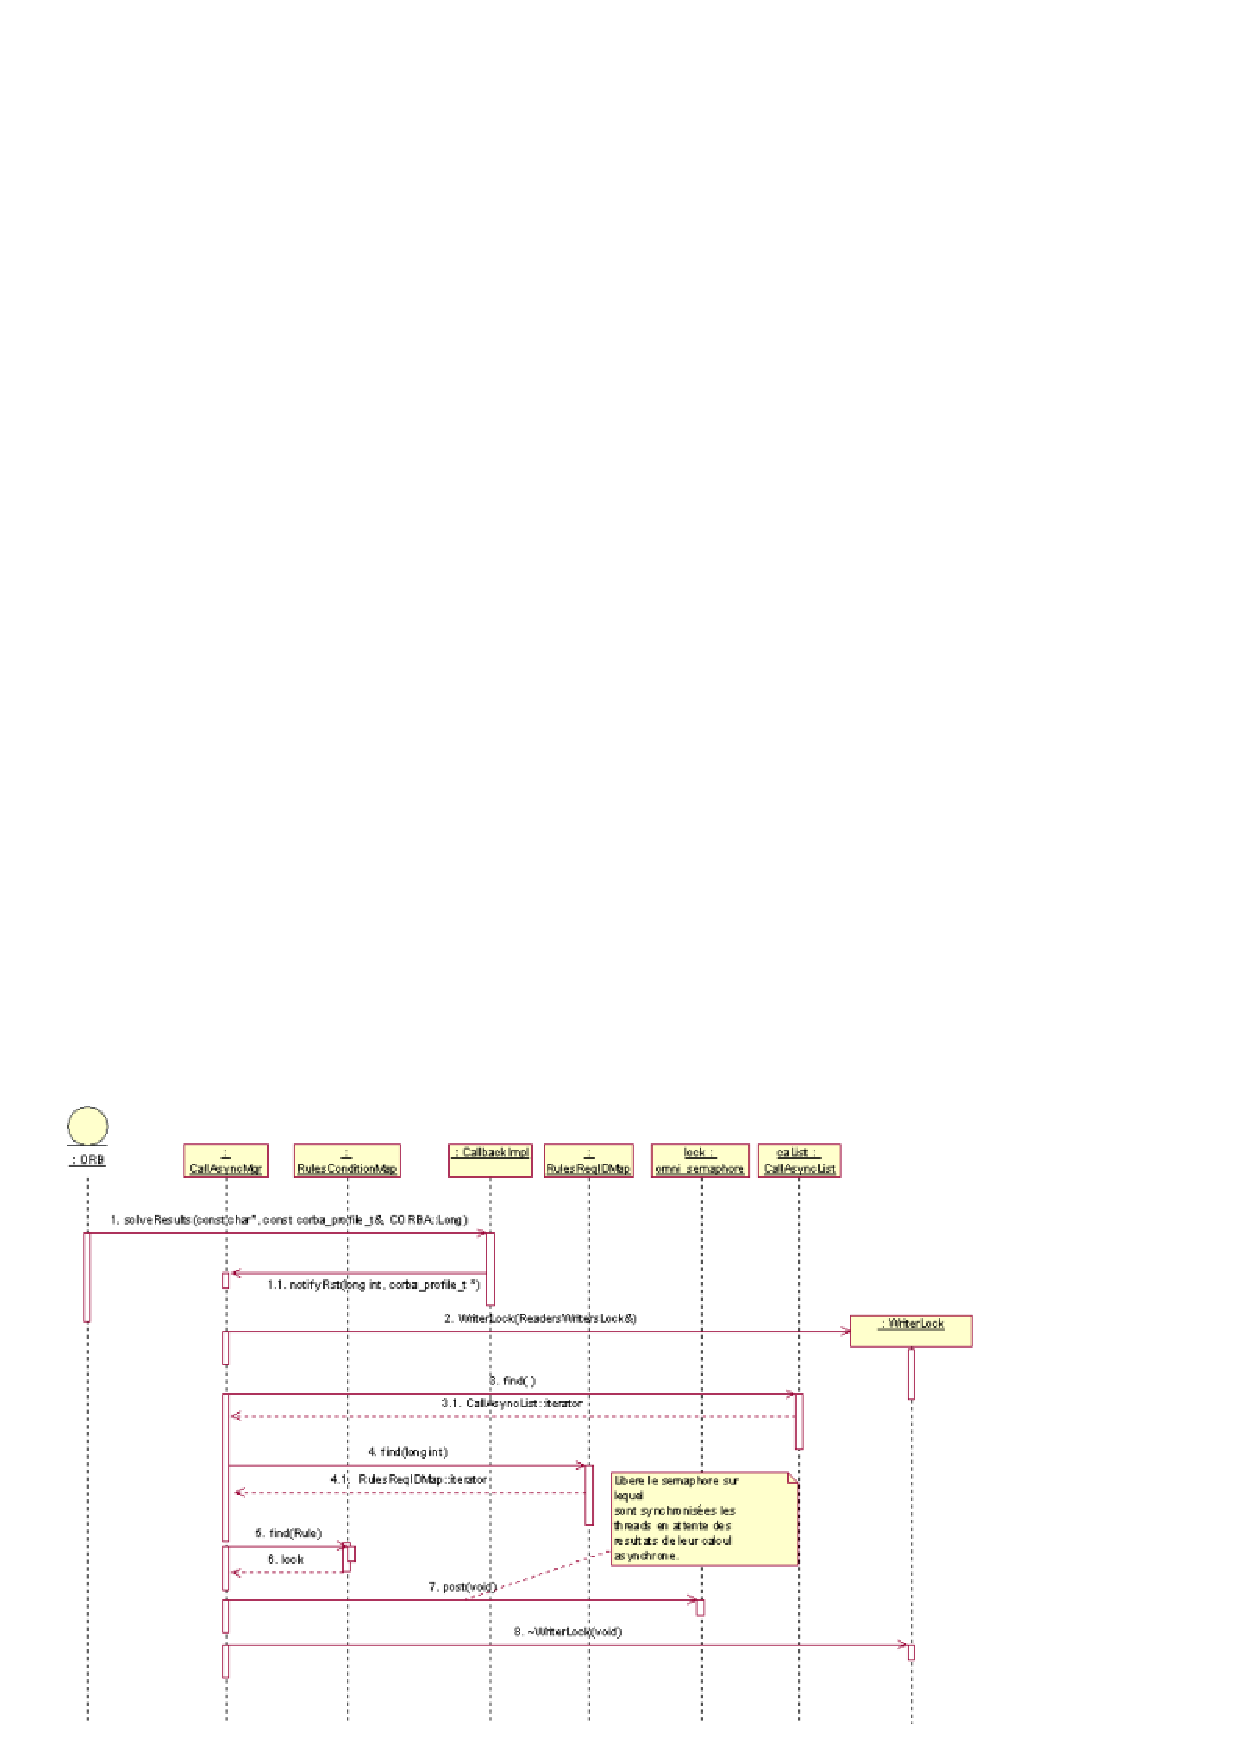
\includegraphics{./fig/CallbackSynchronisationSequenceDiagram}
  \end{center}

  \begin{itemize}
  \item SeD pushes results on client by a CORBA call to \emph{solveResults}.
  \item Callback server notifies available results by a call to \emph{notifyRst}.
  \item locks synchronising mecanism (\emph{WriterLock}).
  \item validates data and request identifier(\emph{find}).
  \item finds rules linked to retrieved results.
  \item verifies all rules waiting conditions.
  \item unlocks waiting threads linked to these rules.
  \item unlocks synchronising mecanism (\emph{~WriterLock}).
  \end{itemize}

  \subparagraph{Getting result state by an asynchronous function:}
  Unlike local synchronous call as \emph{addWait*}, client can get results
  state with \emph{getStatusReqId}. This call returns an enum type \emph{STATE}
  which defines five state (RESOLVING, WAITING, DONE, CANCEL, ERROR).
  \emph{CallAsyncMgr::addWait*} returns also this enum.
  RESOLVING announces that calculus goes on, WAITING that is not started,
  DONE that is finished and results are availabale, CANCEL that is stopped
  by user and ERROR that is stopped by an error or an exception.

  \begin{center}
  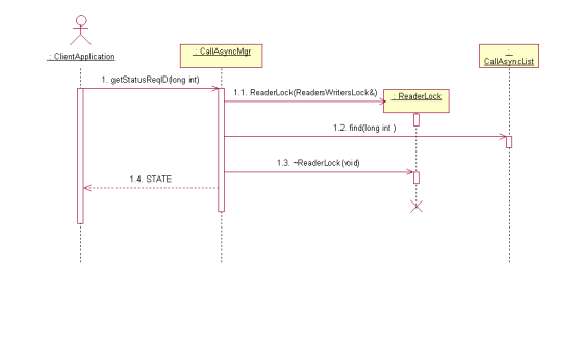
\includegraphics{./fig/CallAsyncProbeSequenceDiagram1}
  \end{center}

  \begin{itemize}
  \item call of \emph{CallAsyncMgr::getStatusReqId}.
  \item lock synchronising mecanism.
  \item verify calculus identity and validity.
  \item get state linked to calculus.
  \item unlock synchronising mecanism.
  \end{itemize}

  \noindent
  \fbox{\textbf{NB}} This algorythm is also used by \emph{diet\_probe} function
  into GridRPC API.

  \subparagraph{Managing memory in asynchronous request:}
  \emph{CallAsyncMgr::deleteAsyncCall} frees internal data linked to a
  calculus if it is finished, its results are available and no rule includes
  it into its waiting conditions.
  If others rules are linked to this result, their state are modified to
  CANCEL as well as calculus state linked. Then synchronising mecanisms
  are unlocks, threads goes on and \emph{CallAsyncMgr::addWait*} returns
  CANCEL state. Finally, memory is free.

  \begin{center}
  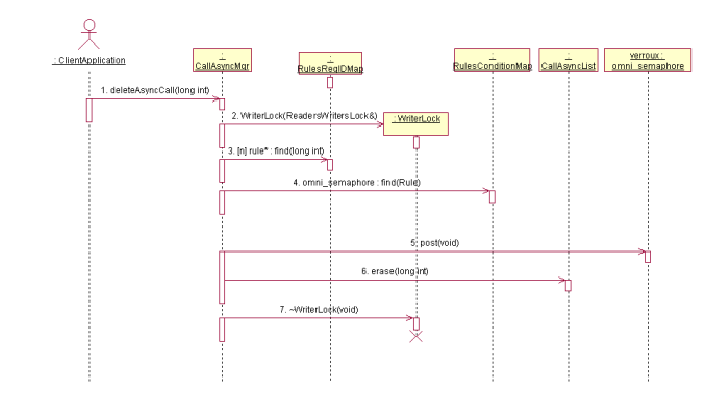
\includegraphics{./fig/DietCancelSequenceDiagram}
  \end{center}

  \begin{itemize}
  \item call of \emph{callAsyncMgr::deletecallAsync}.
  \item lock synchronising mecanism.
  \item verify request identifier.
  \item look for rules linked to request identifier,
  unlock synchronising items and fix rule state with CANCEl.
  \item free memory alocated to rule data and mutexes.
\item free data about request (request identifier, state, ...)
  \end{itemize}

  \noindent
  \fbox{\textbf{NB}} These algorythms only concern client processus. Next development steps
  will provide direct interactions to SeD server processus using persistence
  service.

  \section{\textsf{src/CORBA}}
  \label{s:CORBA}

  \subsection{\textsf{ORBMgr}}

  This module has been written to hide the ORB to the rest of the code. The idea
  is that every ORB-dependent operation might be performed through a unified API,
  described in \textsf{ORBMgr.hh}. Of course, DIET still supports only omniORB,
  but soon it should support TAO too.
  \\
  This module does not aim at unifying the APIs of the various thread libraries of
  such ORBs. As this should be a part of the DIET API, it should be processed in
  what \textsf{DIET\_mutex} could become.
  \\
  It has been decided to add to this module some of the usual OMG calls, so that
  it is easier to initialize, bind its name in the naming service, etc.


  \subsection{Data memory management}

  \fixme{Bruno - Help me please, if I have no time ...}


  \subsection{Convertors}

  \fixme{under construction ...}



  \section{\textsf{src/CORBA/idl}}
  \label{s:IDL}

  In this directory, all IDL interfaces have been gathered. They are organized as
  follows:
  \begin{description}
  \item {\sf common\_types.idl}: all (almost all) types used in all the
  communications of the platform.
  \item {\sf response.idl}: the structure of a response, with the sorted
  (scheduled) lists of servers.
  \item {$[$\textsf{Local$|$Master}$]$\textsf{Agent.idl}, \textsf{Callback.idl} and \textsf{SeD.idl}}: the interfaces of the CORBA objects of the hierarchy.
  \end{description}
  Note that the type \texttt{corba\_estimation\_t} should be declared in
  \textsf{response.idl}, since it is a part of a response. But this would
  introduce a crossed-dependency: \textsf{response.idl} includes \textsf{SeD.idl}
  because a response contains the references to the servers, and \textsf{SeD.idl}
  needs the \texttt{corba\_estimation\_t} to be declared for the method
  \textsf{checkContract}. So, to get rid of the crossed-dependency, the type is
  declared in \textsf{common\_types.idl}.
  \\

  Compiling the IDL interfaces is a bit more complex than for any C or C++ file.
  Automake has no mechanism to manage IDL files, except the
  \texttt{BUILT\_SOURCES} variable. This variable stores all the C++ files
  generated by the compilation of the IDL files\footnote{The names of these files
    depend from the IDL compiler, but most of the compilers let the user choose
      the nomenclature}. But we must still specify the dependencies of the built
      sources from the IDL files. This is the role of the file \textsf{idlRules.mk}.

      \textsf{idlRules.mk} is included in Makefile.am defining compiling and linking rules
      with idl generated stubs files ( with omniORB, xxSK.cc and xxDynSK.cc). It contains
      a list of idl files, rules, targets, list of cleaned files and fixes a python
      bug.

      %    \fixme{Christophe - Explain the \textsf{idlRules.mk} - its role in the
        %     compilation chain}


        \section{\textsf{src/examples}}
        \label{s:examples}

        This directory contains the examples distributed with DIET. Its compilation
        depends on the configure option \texttt{--enable-examples}, forced in
        maintainer, and disabled by default for users.

        There are five complete applications, providing a server and one or several
        clients able to use the service(s) offered by the server. Two of them require
        special libraries to be installed on the machine, which are more or less
        detected at configuration time, but there is still much work to do for
        the automatic detection.

        \subsubsection{file\_transfer}

        This example was aimed to show how to manipulate the \texttt{DIET\_FILE} type.
        The client sends two files to the server. The second file is re-transfered
        without any change, since it is an INOUT, and its size is returned as an OUT.
        It shows the drawback of the file management: it is impossible for the user to
        gain control over the path of the received files.

        \subsubsection{scalars}

        This example was aimed to show how to manipulate the \texttt{DIET\_SCALAR} type,
        and the various modes of passing arguments. It shows the problems of the
        management of the base types in DIET: the length of the given data is not
        checked, and the correspondance with the CORBA types is still to be perfected.
        Actually, the length of the base types has been defined according to the
        NetSolve types, but it would have been more clever to accord them with the CORBA
        types.

        \subsubsection{dmat\_manips}

        The server offers an interface to some basic double matrix manipulations:
        transpose, product and sum. To make the clients of the examples
        \texttt{dmat\_manips}, \texttt{BLAS} and \texttt{ScaLAPACK} interchangeable for
        some problems, the profiles for services \texttt{MatPROD}, \texttt{SqMatSUM}
        (square matrix sum) and \texttt{SqMatSUM\_opt} (``optimized'' because the second
                                                        operand is INOUT) are the same. Thus, for a demo, a matrix product can be
        invoked by a client, and executed either on a server having the BLAS library
        installed, or a server performing only a basic matrix product (usually far much
            slower), according to the FAST estimation.
        \\

        Although there are many examples of convertors in this and other examples, the
        service \texttt{T}, the first written, was designed to give an example of
        remanipulation of the arguments. When FAST 0.4 has been integrated into DIET,
        all other services had to include convertors.

        Another step has been done for FAST 0.8. The convertors had to be rewritten
        since the matrix type has been suppressed from the FAST API (with all high-level
            descriptions of the problems) The idea is to create a profile, through the
        convertor, that has got only the arguments declared in the LDAP base (which can
            be extracted from the others), followed by the arguments that the computation
        needs. It was not possible to do that with FAST 0.4 because it was not designed
        to ignore unknown arguments. That is why we are forced to include
        \textsf{DIET\_config.h}, to get the version of FAST.
        \\

        %\fixme{Christophe - Please explain the asynchronous clients.}
        \texttt{dmat\_manips} contains also client samples about asynchronous call API. All
        use \texttt{diet\_call\_async} to start solve on SeD but each example shows
        a distinct function of asynchronous DIET API to get results. Like synchronous
        client, you can ask solving a SUM/PROD/T operation on SeD. Besides, they are
        \texttt{multithreaded}. You can specify thread number of a pool and solve number. Each
        thread cucurently sends data to SeD(s) and gets results according to its used
        \texttt{diet\_wait\/probe\_*} function.
        \texttt{parallelclient.cc} retrieves results by a simple \texttt{diet\_wait} function
        and \texttt{parallelclient2.cc} by a peridical \texttt{diet\_probe} call.
        \texttt{parallelclient3.cc} and \texttt{parallelclient3.cc} are examples about
        respectivly \texttt{diet\_wait\_and} and \texttt{diet\_wait\_or}. Executing
        one of these examples prints traces about calculus parameters, synchronizing
        mecanisms on threads and results.

        \subsubsection{BLAS}

        To compile the BLAS server, you will need the BLAS library installed. For
        developers using a Linux Debian, there is a package, and everything has been
        performed for the configure to take such a package into account: just use the
        \texttt{--enable-BLAS} option, and it should be automagically detected. For
  other installations, it might be necessary to use all the arguments defined by
the ACI\_PACKAGE macros (\texttt{--with-BLAS=}, ...)

  So far, this server provides the \texttt{dgemm} service and all its derivations:
  \texttt{MatPROD}, \texttt{SqMatSUM}, \texttt{SqMatSUM\_opt} and
  \texttt{MatScalMult}. Convertors are used to convert the profiles of the
  problems to the one of the pdgemm service, so that only one solve function has
  to be implemented. But this server is destined to be an interface to all the
  functions of the BLAS library.
  \\

  We have the same problem of compatibility with FAST 0.4 and FAST 0.8 in the BLAS
  server as in the dmat\_manips example. Actually, this server only supports
  FAST 0.4, since the modifications to get low-level profiles for FAST 0.8 have not
  been done yet. But these modifications are quite similar to the ones of the
  dmat\_manips server, and they will be easy to add.

  \subsubsection{ScaLAPACK}

  It is very difficult to detect all the libraries necessary to compile a program
  calling the \texttt{pdgemm} function. Nothing has been done actually for it in
  the \texttt{configure.ac}, because not only the LAPACK library should be found,
  but also an MPI implementation, etc. Nevertheless it is still possible to
  compile the server of this example if the user knows exactly all the paths for
  these libraries, or the extra arguments to compile with them (through
      \texttt{--with-ScaLAPACK-extra}), thanks to the \texttt{ACI\_PACKAGE} macros
  from M. Quinson.

  So far, this server provides the \texttt{pdgemm} service and all its
  derivations: \texttt{dgemm}, \texttt{MatPROD}, \texttt{SqMatSUM},
  \texttt{SqMatSUM\_opt} and \texttt{MatScalMult}. Convertors are used to convert
  the profiles of the problems to the one of the pdgemm service, so that only one
  solve function has to be implemented. But this server is destined to be an
  interface to all the functions of the ScaLAPACK library.

  The implementation of this SeD is complex. It is launched on the node 0 of an
  MPI grid. When the client submits a problem, it asks for a number of nodes to
  execute the computation. Then, the node 0 creates a subgrid of the available
  nodes and launches the computation on this new grid. Of course, depending on the
  number of nodes required by the client, and the number of nodes still available
  in the initial grid, it is possible that the computation returns with an error
  code, or that the same node is used for several processes.
  \\

  The support for FAST is quite difficult to add, since the server is supposed to
  be parallel. Maybe we should wait for the FAST/Freddy integration to be
  complete.



  \section{\textsf{src/SeD}}
  \label{s:SeD}

  This directory contains the implementations of
  \begin{itemize}
  \item the DIET server API,
  \item the IDL interface of the SeD.
  \end{itemize}
  \

  The functions of the API are easy to understand, as far as the User's Manual is
  well understood. They use a global static variable \texttt{SRVT}, and its
  manipulation is not thread-safe, since it would have no sense to launch two SeDs
  with the same service table in two different threads.
  \\

  There is nothing else important to explain in the implementation of the IDL
  interface but the \texttt{solve} methods. These methods run on the same
  scheme, except that \texttt{solveAsync} is \textit{oneway}, ie. asynchronous,
  and thus it has to send explicitly the results, through a callback mechanism, at
  the end of the computation.

  %\fixme{Christophe - the callback mechanism might require some more explanations}
  In case of asynchronous call, i.e solve\_async call, client specifies a request
  identifier and a CORBA reference defining its Callback client server (IP/Port).
  And thus, at the end of the solve, the \texttt{solveAsync} function call \texttt{notifyRst}
  of client callback server with diet profile and request ID parameters. Client manages
  callback threads, results and notifying news through its asynchronous API.
  After this calling, SeD thread free memory.

  Both methods have to ``unmarshall'' the arguments, ie. to convert them into DIET
  data that the programmer of the server can manipulate. Then they invoke the
  solve function through the pointer given by this programmer, and reconvert
  (marshall) the OUT data into CORBA data to be sent back on the client. Thus the
  computation is performed inner a CORBA thread, created at the remote invokation
  of the method.

  To perform the computation in a separate process, we will be forced to dump the
  arguments into files ... It is still to be done.


  \section{\textsf{src/utils}}
  \label{s:utils}

  This directory gathers all tools and utils that are used by more than one
  entity of DIET.

  \fixme{under construction ...}

  \subsection{\textsf{Counter}}

  The \texttt{Counter} class implements a thread safe counter. This counter
  accepts only 32 bits positive value. This class must be used each time a
  counter is shared by several threads. Read the doxygen documentation for more
  informations about how-to use it.

  \subsection{\textsf{ms\_function}}

  Several calls to \texttt{strdup()}, \texttt{CORBA::string\_dup()},
  \texttt{malloc()} and \texttt{stralloc()} are made inside the DIET code. The
  problem is : each of these functions can return the \texttt{NULL} value. The
  use of an allocated memory without testing the \texttt{NULL} value will
  probably result to a segmentation fault if there was not enough memory. This
  is why the \textsf{ms\_function} file describes some functions which allocate
  the memory and test if the \texttt{NULL} value is returned. If it is the case,
  a \texttt{bad\_alloc} exception is thrown, if not the functions behave like the
  standard ones. Read the doxygen documentation for more informations about
  how-to use them.

  \subsection{\textsf{ts\_container}}

  The C++ Standard Library gives access to several containers. A map, a vector, a
  list and a set templates are defined by the C++ Standard. The only problem with
  them is that there are not thread safe. If two threads alter a container at the
  same time, a crash is on the way. Therefore a critical section access mechanism
  must be implemented to avoid it. It is easy to forgot to lock the access to a
  list before using it. This is why the \texttt{ts\_container} exists (the
      \texttt{ts} is for Thread Safe). They managed the access to there critical
  section by themselves. All the list and set which are shared by several threads
  must be implemented with a \texttt{ts\_container} to avoid a simultaneous
  access to it. Read carefully the doxygen documentation to know which one to use
  and how-to use it.

\section{\textsf{Cmake}}
\label{s:Cmake}

This directory gathers the cmake related scripts that cmake authorizes to
be deported here.



%
% Coding Standards
%
\chapter{Coding Standards}
\label{ch:CS}
%****************************************************************************%
%* DIET Coding Standards - chapter three of the Programmer's Guide          *%
%*                                                                          *%
%*  Author(s):                                                              *%
%*    - Philippe COMBES (Philippe.Combes@ens-lyon.fr)                       *%
%*                                                                          *%
%* $LICENSE$                                                                *%
%****************************************************************************%
%* $Id$
%* $Log$
%* Revision 1.5  2007/11/22 21:07:02  mimbert
%* use latex package fancyhdr instead of fancyheadings which seems deprecated in some recent latex distributions
%*
%* Revision 1.4  2006/12/06 10:00:24  eboix
%*  Coding style comments added for CMakeLists.txt. This is just a reminder
%*  of existing rules, but it will authorize even further punishment for the
%*  ones breaking them. Caveat emptor... --- Injay2461 getting anal on this.
%*
%* Revision 1.3  2003/12/02 10:29:02  sdahan
%* update the doxygen part of the Programmer Guide
%*
%* Revision 1.2  2003/09/17 14:41:28  pcombes
%* Split the .tex according to its chapters.
%*
%* Revision 1.1  2003/09/09 12:42:44  pcombes
%* Reorganization of doc: include CS in a programmer's guide.
%*
%* Revision 1.9  2003/06/03 18:22:05  pcombes
%* License field is kept.
%*
%* Revision 1.8  2003/04/10 11:12:43  pcombes
%* Put the CVS Id field right above the CVS Log field.
%*
%* Revision 1.7  2003/02/07 15:32:49  pcombes
%* Update - noting new in the background
%*
%* Revision 1.3  2003/01/30 15:13:42  pcombes
%* New Coding Standards
%*
%* Revision 1.2  2003/01/13 12:09:00  pcombes
%* UM: client part complete for users's day ...
%*
%* Revision 1.1.1.1  2003/01/07 18:06:18  pcombes
%* Add Coding Standards for DIET.
%****************************************************************************%

\begin{comment}
\documentclass[11pt,a4paper]{article}
\makeatletter
%\makeatother
\usepackage{fancyhdr}
%\usepackage[french]{babel}
%\usepackage[latin1]{inputenc}
\usepackage{multicol}
\usepackage{verbatim}
\usepackage[headings]{fullpage}
\usepackage{url}

\usepackage{graphicx}
\graphicspath{{../UM/fig}}

\newsavebox{\logobox}
\sbox{\logobox}{
\includegraphics[scale=0.3]{../UM/fig/logo_DIET.ps}}
\newcommand{\logo}{\usebox{\logobox}}

%%%%
\renewcommand{\title}{DIET Coding Standards}
%%%%

\pagestyle{fancyplain}
\lhead[\fancyplain{\title}{\title}]
      {\fancyplain{\title}{\title}}
\chead{}
\rhead[\fancyplain{\logo}{\logo}]{\fancyplain{\logo}{\logo}}

\lfoot[\fancyplain{INRIA}{INRIA}]{\fancyplain{INRIA}{INRIA}}
\cfoot[\fancyplain{}{}]{\fancyplain{}{}}
\rfoot[\fancyplain{Page~\thepage}{Page~\thepage}]
      {\fancyplain{Page~\thepage}{Page~\thepage}}


\begin{document}
%\vspace*{1cm}
\thispagestyle{empty}
\begin {center}
\noindent\textbf{\LARGE{\title}}
\end{center}
\vspace*{1cm}
\end{comment}

In a continuous attempt to unify the structure and the format of the DIET source
code, we have collected a few guidelines here to which we ask you to adhere as
you add new source code or modify the existing code. We ask you to make every
effort to follow our guidelines before you submit your contributions to the
project. We also ask for your help in improving existing incompliant code as you
make modifications to it.


\section{File structure}
\label{fstruct}

\subsection{Headers}

Each file begins with the DIET header, where are precised:\\
\begin{tabular}{l}
- a short title (in one line)  that explains the role of this file (l. 3),\\
- the authors of the file,\\
- three fields that are automatically filled in.\\
\end{tabular}

As an example, here is the header of the \LaTeX\ source of this document, before
\texttt{\$Id\$} and \texttt{\$Log\$} fields have been filled in by CVS
operations:
\footnotesize
\begin{verbatim}
%****************************************************************************%
%* DIET Coding Standards                                                    *%
%*                                                                          *%
%*  Author(s):                                                              *%
%*    - Philippe COMBES (Philippe.Combes@ens-lyon.fr)                       *%
%*                                                                          *%
%* $LICENSE$                                                                *%
%****************************************************************************%
%* $@Id$
%* $@Log$
%****************************************************************************%
\end{verbatim}
\normalsize
% NB: in the verbatim above, the $@ is replaced by $ before the latex
%     compilation to produce the correct output. If we did not use such an
%     artefact, the cvs commits would fill in fields also ...

The CMakeLists.txt are not submitted to this header marking (since it was
considered that there is no technical value attached to them).


The fields \texttt{\$Id\$} and \texttt{\$Log\$} are automatically set at every
CVS commit on the file. The CVS log message is added to the \texttt{\$Log\$}
region, prefixed by the characters that preceeds \texttt{\$Log\$} on its line.
It thus keeps the history of all modifications performed on the file. But it may
increase drastically the size of the file with some useless information. So
please help us purging sometimes this Log part of all minor modifications (such
as bug fixes).

These CVS fields are removed by a shell script when a distribution is built. The
\texttt{\$LICENSE\$} line will also be processed automatically, o be replaced by
a short version of the DIET license, so please be very careful to put one and
only one space between the \texttt{\%*} and the \texttt{\$}, between
\texttt{\$Id\$} and the final \texttt{*\%}, between \texttt{\$LICENSE\$} and the
final \texttt{*\%}, and NO space after the last
significant character of all these lines.

\subsection{Defining a new class}

In a class declaration, the public part comes before the private one. Inner each
part, declare the field first, and all methods then.

The file in which the class is declared should be named
\texttt{$<$ClassName$>$.hh} and the one in which it is implemented should be named 
\texttt{$<$ClassName$>$.cc}.


\section{Naming}

Please follow the chapter 9 of the JAVA coding conventions.

\subsection{Classes}

Class names should be nouns, in mixed case with the first letter of each
internal word capitalized. Try to keep your class names simple and descriptive.
Use whole words-avoid acronyms and abbreviations (unless the abbreviation is
much more widely used than the long form, such as URL or HTML).
\footnotesize
\begin{verbatim}
class AgentImpl
{
  ...
\end{verbatim}
\normalsize


\subsection{Methods}

Methods should be verbs, in mixed case with the first letter lowercase, with the
first letter of each internal word capitalized.
\footnotesize
\begin{verbatim}
run();
addServices();
\end{verbatim}
\normalsize


\subsection{Member Variables}

Member variable names should be short yet meaningful. The choice of a variable
name should be mnemonic - that is, designed to indicate to the casual observer
the intent of its use.
\footnotesize
\begin{verbatim}
float myWidth;
\end{verbatim}
\normalsize


\subsection{Variables}

All instance, class, and class constants are in mixed case with a lowercase
first letter. Internal words start with capital letters.\\

Variable names should not start with underscore \texttt{\_} or dollar sign
\texttt{\$} characters, even though both are allowed. They can follow the
members naming conventions or be lowercase with words separated by underscores.
One-character variable names should be avoided except for temporary "throwaway"
variables. Common names for temporary variables are i, j, k, m, and n for
integers; c, d, and e for characters.
\footnotesize
\begin{verbatim}
int   i;
char* c;
\end{verbatim}
\normalsize


\subsection{Constants and Macros}

The names of variables declared class constants and of ANSI constants, the names
of macros and enum constants should be all uppercase with words separated by
underscores. (ANSI constants should be avoided, for ease of debugging.)
\footnotesize
\begin{verbatim}
#define TRACE_STRUCTURES 10
static int MIN_WIDTH = 4;
typedef enum {
  DIET_CHAR,
  ...
}
\end{verbatim}
\normalsize


\subsection{Types}

Type names must be suffixed with \texttt{\_t}: \texttt{diet\_type\_t}.



\section{Comments and Documentation}

Source code documentation is essential in an increasing group of developers
producing software collabortatively and efficiently.

\subsection{Source code}

Comments within the source code are one way to create a comprehensive
documentation. This insures that the related information is in the right place
and makes it easier for the software engineer to maintain it.

Inside DIET we use line comments to describe certain attributes, block comments
to explain bigger code sections and Doxygen comments to declare modules,
functions and other important parts of the software.

Line comments look like this:
\footnotesize
\begin{verbatim}
  int reqId;      /* Request ID */
or
  int reqId;      // Request ID
...
  } else { /* At least one offered service matches the problem */
or
  } else { // At least one offered service matches the problem
\end{verbatim}
\footnotesize

They are at the end of a line after the code or in the line before it just
like block comments as shown below:
\footnotesize
\begin{verbatim}
    /* Add the new log to the list */
    requestsLog->logMutex.lock();
    requestsLog->append(newLog);
    requestsLog->logMutex.unlock();
\end{verbatim}
\normalsize
\noindent \textbf{NB:} All comments are written \texttt{in english} !!!\\

It can be introduced a hierarchy in comments by the use of various symbols. For
instance, some comments can be used to simply separate the file into main
sections that group functions or methods together:
\footnotesize
\begin{verbatim}
  /****************************************************************************/
  /* Private methods                                                          */
  /****************************************************************************/
or
  /****************************************************************************/
  /* Data structure marshalling                                               */
  /****************************************************************************/
\end{verbatim}
\normalsize

Each method or function must be commented with Doxygen comments (see below)
Inside functions or methods, you can use '//' to mark that the comment is less
important than '/* ... */' comments.
\\


Eventually, please comment even your \verb+#if+ an \verb+#ifdef+ conditions: add
the conditional expression as a comment on the corresponding \verb+#else+ and
\verb+#endif+ lines:
\footnotesize
\begin{verbatim}
#if HAVE_FAST
  ...
#else  // HAVE_FAST
  ...
#endif // HAVE_FAST
\end{verbatim}
\normalsize

\subsubsection{Doxygen}

\textit{Doxygen} is a documentation system very similar to javadoc. It analyses
the header files of your code and build a pretty and easy to use documentation
from it. You can/must add some comments into your header file to describe the
interface of your classes. If the comment start by \texttt{/**} instead of
\texttt{/*}, \textit{Doxygen} takes it as the description of your class or
method. The documentation of Doxygen can be found at
\url{http://www.stack.nl/~dimitri/doxygen/docblocks.html}.

The most important things that must be put in the documentation is the
hypothesis made by our methods. If your class can accept several modifications
in the same time, you put ``this class is thread safe'' in the
documentation. If a methods accept a \texttt{char*} as a parameter but not the
\texttt{NULL} value, the documentation must say it too. It is useless to put
tons and tons of documentation, but nothing must stay undefined and an example
of use can be useful. This is really important when you describes your methods,
every hypothesis about your parameters and the state of the object must be
defined.

The easiest way to learn how to use \textit{Doxygen} is to look at a header
with \textit{Doxygen} comments like the \texttt{src/utils/Counter.hh} file. To
build the documentation run \texttt{doxygen doc/Doxyfile} in the source
directory of diet. The API directory will be created with all the
documentations inside. There is one rule that you must remember : always put
your comment just above your prototype or it will be ignored by
\textit{Doxygen}.

As there are C files in the DIET sources, the flag \texttt{@author} cannot be
used in all DIET source files. Thus, it is important to identify the author
of the file \textbf{in the header}, as explained section \ref{fstruct}.  Using
the flag \texttt{@author} would be redundant.

One last thing, do not put some \texttt{//FIXME blablabla} but use \texttt{/**
@warning blabla */}, \texttt{/** @todo blabla */} and \texttt{/** @bug blabla
*/} directly in the C code. A report will be generated with all the todo,
warning and bugs. It will be easier to know what must be done.

\subsection{Manuals}

As soon as modifications visible from the user's point of view are performed,
they have to be commented in the \textit{User's Manual}. These include changes
in the installation process, in the API or still in the general behaviour of the
platform, the new features that a programmer could add, etc. The \textit{Users's
  Manual} should always be up-to-date.
\\

It is also very important for the developers to maintain this
\textit{Programmer's Guide}, essentially the first two chapters of course.
Indeed, these chapters expose the architecture of the software, its various
parts and their links: this could evoluate a lot with the future developments.
The \textit{Programmer's Guide} is not redundant with the comments put into the
source code, since these comments cannot give a general view of the software,
and some parts of the code require so many comments that it is better to put
them in this \textit{Programmer's Guide}, with a simple reference in the
source code. Moreover, it is a \textit{guide}, which means it should help a
newbie programmer finding quickly what changes to do and where, before having
read the least source code line.


\section{Tabs, Line Length and Indentation}

Please do not use tabs inside of the code and wrap lines after the 80th
character in a line. We do not like tabs because different editors and editor
settings always lead to different displays. However, it is permitted to insert
tabs if and if only they correspond to 8 charcters in the indentation (as for
GNU-Emacs standards).

Lines have to be indented by two spaces for each code block level.  See more
details below, especially in section \ref{s:statements}.

Due to cmake's syntax design choices \texttt{CMakeLists.txt} tend to
quickly feed the 80 characters width of a line. For \texttt{CMakeLists.txt}
files it was thus chosen to use a 2 or 3 characters indentation width.
If we strictly conform to the above limited-tabs recommendation,
\texttt{CMakeLists.txt} should thus remain tab free.

\section{Declarations}


\subsection{Variables}

Initialize variables at declaration. It is accepted not to initialize
"throwaway" variables, and to declare several of them on one single line.

The asterisk of a pointer declaration and the \texttt{\&} of a reference
declaration are parts of the \textbf{type} name. The space has to be put in
between the \texttt{*} or the \texttt{\&} and the type name.
\footnotesize
\begin{verbatim}

\end{verbatim}
\normalsize

\subsection{Functions}

The format of a function prototype should be equivalent with the function
definition. Return type and keywords such as extern, static, export, explicit,
inline, etc, go on the line above the function name. They should start with the
qualifier and return type. There is no space between the function name and the
open parentheses. If the arguments do not fit into one line split the line and
continue the arguments under the first one of the previous line.

\footnotesize
\begin{verbatim}
CORBA::Long
AgentImpl::serverSubscribe(SeD_ptr me, const char* hostname,
                           const SeqCorbaProfileDesc_t& services)
{
�� ...
or
int
unmrsh_in_args_to_profile(diet_profile_t* dest, corba_profile_t* src,
                          const diet_convertor_t* cvt)
{
�� ...
\end{verbatim}
\normalsize

\noindent In the function definition, the brace has to be in column zero again.
\footnotesize
\begin{verbatim}
int
mrsh_profile_to_out_args(corba_profile_t* dest, const diet_profile_t* src,
                         const diet_convertor_t* cvt)
{
  int i, res;
  int arg_idx(0);
  int* args_filled = new int[(dest->last_out + 1)];
  diet_data_t dd;
� ...
\end{verbatim}
\normalsize


\section{Statements}
\label{s:statements}

Statements inside the function body should be indented with 2 spaces like
statements inside a compound statement.  In contrast to functions, the opening
left brace of a compound statement should be at the end of the line beginning
the compound statement and the closing right brace should be alone on a line.
Some examples:\\

\footnotesize
\begin{center}
 \begin{tabular}{l|l}
  \begin{minipage}[c]{.5\linewidth}
   \begin{verbatim}
  for (int i = 0; i < max_nb_s; i++) {
    ...
  }

  do {
��    ...
  } while (!found);



  if (i == 1) {
��    ...
  } else if (i == -5) {
��    ...
  } else {
��    one_function_call();
  }

   \end{verbatim}
  \end{minipage}
&
  \begin{minipage}[c]{.5\linewidth}
   \begin{verbatim}
  while (1) {
��    ...
  }
  
  switch (i) {
  case 1,2:
��    ...
��    break;
  case 3:
��    ...
��    break;
  default:
��    ...
  }

  typedef struct name_s {
��    char *first;
  } name_t
   \end{verbatim}
  \end{minipage}\\
 \end{tabular}
\end{center}

\textrm
\normalsize

There is one space between the keyword and the open parentheses. Braces are in
the same line like the keywords. They should be used even if it is not
necessary. Function calls do not contain spaces between the function name and
the open parentheses.

\section{Clean use of C++ constructs}

Past experience leads us to some best-practice coding advices:
\begin{itemize}
\item Huge parameter lists or function or methods bodies are an indicator that
  it is time to split a function or method into some smaller ones which are
  easier to read and understand.
\item Try to avoid nested expressions where multiple assignments or the
  $?$-operators are envolved.
\item Use \verb+#if 0+ to disable code sections and add a short comment why this
  code was disabled.
%\item Avoid casting a CORBA type variable with a C/C++ type.
\end{itemize}

%\end{document}



%
% Remarks and Batch jobs
%
\chapter{Batch Submission and general remarks}
\label{ch:Batch}
%****************************************************************************%
%* DIET Programmer' guide, batch/parallel submissions                       *%
%*                                                                          *%
%*  Author(s):                                                              *%
%*    - Yves Caniou (yves.caniou@ens-lyon.fr)                               *%
%*                                                                          *%
%* $LICENSE$                                                                *%
%****************************************************************************%
%* $Id$
%* $Log$
%* Revision 1.10  2008/04/07 22:26:26  ecaron
%* Updated files to pdflatex compilation
%*
%* Revision 1.9  2006/11/30 14:14:16  ycaniou
%* diet -> textsc{Diet} (Tkx Abdelkader)
%*
%* Revision 1.8  2006/11/30 13:58:07  aamar
%* Remove an extra \
%*
%* Revision 1.7  2006/11/28 20:40:30  ycaniou
%* Only headers
%*
%* Revision 1.6  2006/11/27 08:13:58  ycaniou
%* Added missing fields Id and Log in headers
%****************************************************************************%

This chapter contains things that must be dispatched along the
programmer's guide (and even more detailed?). It is actually in
writing, and contains, for the most, remarks.\\

The concern of this chapter is parallel and batch submission and how
we achieve to do it in \textsc{Diet}. In consequence, it deals with
choices made for the API, with all the structures which are used in
the recording of problems and the submission of jobs, and with all the
mechanisms which are involved. Tools on which we rely, like Elagi and
Appleseeds are also mentionned.

%****************************************************************************%
\section{Notations in pseudo code parts and terminology}
%****************************************************************************%

\subsection{Notations in pseudo-code}

``.fonction()'' is written to know rapidly it is a call. If a
tabulation appears after, then the following describes the called
fonction. Should be replaced by UML graphs.

\subsection{Terminology (taken from the User manual)}

Because a good understanding comes with correct terms, we provide here
the definition of the terms that we will use thereafter.

Servers provide {\it services}, e.g instanciation of {problems} that a
server can solve: for example, two services can provide the resolution
of the same problem, one being sequential the other parallel. A
\textsc{Diet} {\it task}, also called a {\it job}, is created by the
{\it request} of a client: it refers to the resolution of a service on
a given server.

A service can be sequential or (exclusive) parallel, in which case its
resolution requires numerous processors of a parallel resource (a
parallel machine or a cluster of workstation). If parallel, the task
can be modeled with the MPI standard, or composed of multiple
sequential tasks (deployed for example with \verb!ssh!) resolving a
single service: it is often the case with data parallelism problems.

Note that when dealing with batch reservation systems, we will likely
speak about {\it jobs} rather than about {\it tasks}.

%****************************************************************************%
\section{Notes on structures}
%****************************************************************************%

\subsection{Generalities}
\begin{itemize}
\item A changement in a structure which has to be transfered: CORBA
Must look in idl, etc.

\item Conversion between structures is partly done in CORBA/marchalling.cc
\end{itemize}

\section{About parallel and batch jobs}

\subsection{Definition}

The executable of a parallel job is found on the nodes where it has to
be executed, either with the NFS filesystem or because the user has
copied it to all nodes with \verb!scp! for example.

In High Computing, parallel jobs are usually MPI codes, but they can
also be several independent communicant codes. We consider here that
it can be launched by using the correct MPI sequence (depending on the
implementation - MPICH or LAM for example) or by calling one of the
code, which will do the necessary thereafter.

\subsection{Objectives}


\subsection{Configuration and compilation (complementary of the User Manual.}

\subsection{Implementation.}$ $\\
We must put a \textsc{Diet} reqID in the profile because we only know
the batch ID when submitting the script which is built when calling
the function given in the programmer SeD. We need to establish a
correspondance between both IDs, done in the SeD.

\subsection{Main structures: sum-up}
Here, we present the structures used along the recording of problems
and the submission and resolution of tasks. 

Note that the \verb$corba_pb_desc_t$ can be accessed through the
\verb$corba_request_t$ structure.

\newpage

\pagestyle{empty}

\begin{minipage}[h]{.3\linewidth}
\begin{verbatim}
typedef struct {
  char*       pb_name;
  int         last_in, last_inout, last_out;
  diet_arg_t* parameters;

  const void* SeDPtr; /* pointer to SeD object, to be used in
                      ** performance estimation
                      ** And for batch submission */
#ifdef HAVE_BATCH
  unsigned short int batch_flag ;
  int nbprocs ;
  unsigned long walltime ;
  // Used for correspondance batch job ID / DIET job ID
  int dietJobID ;
#endif

} diet_profile_t;
\end{verbatim}
\begin{verbatim}
/** Service profile descriptor (mapping for diet_profile_desc_t) */
struct corba_profile_desc_t {
  string path;
  long   last_in;
  long   last_inout;
  long   last_out;
  sequence<corba_arg_desc_t> param_desc;
#if HAVE_BATCH
  long batch_flag ;
#endif
  corba_aggregator_desc_t aggregator;
};
\end{verbatim}
\begin{verbatim}
/**
 * Actually, this is an equivalent to a diet_profile_t without the data.
 */
struct corba_pb_desc_t {
  string path;
  long   last_in;
  long   last_inout;
  long   last_out;
  SeqCorbaDataDesc_t param_desc;
#if HAVE_BATCH
  long   batch_flag ;
  long   nbprocs ;
  long   walltime ;
#endif
};

/** The complete problem, sent from client to server. */
struct corba_profile_t {
  long   last_in;
  long   last_inout;
  long   last_out;
  SeqCorbaData_t parameters;
#if HAVE_BATCH
  long   batch_flag ;
  long   nbprocs ;
  long   walltime ;

  unsigned long dietJobID ;
#endif
};
\end{verbatim}
\end{minipage}

\newpage

\pagestyle{plain}

\begin{figure}
\begin{center}
\includegraphics[width=14cm]{./fig/DiagrammeGridRPCDietStructure}
\caption{Structures used between GridRPC parts}
\end{center}
\end{figure}

%****************************************************************************%
\section{Notes on recording of services}
%****************************************************************************%

\subsection{Generalities}

Numerous services are statically declared in a SeD. If a server must
provide a problem resolution, either another SeD which can perform it
is launched on the the server or the corresponding SeD is stopped and
another one, whose code has been improved and compiled for the
architecture, is launched.

The code of a SeD can be found in \textsc{Diet}\_server and SeDImpl
files. The first one, written in C, launches a deamon, whose code is
in the second. If you want to add thing to the API, ask yourself if
your changes must consider dynamic stuff (like take into account
CORBA) or is completely static. For example, queues and batch
submission requires dynamic information and therefore are implemented
in SeDImpl.cc.

To add a service, the SeD calls \verb$add_table_service$ and
comparisons are made in order to know if the service is already
declared. Each field is tested!

. addService()
. Each SeD give to the localAgent the list of problems it can solve.
. LocalAgents give their lists to the agent immediately superior in the hierarchy, etc., until the agent is a MA.

$\rightarrow$ This is done to know if it is necessary to transmit a
request on a branch of the hierarchy.

Figure representing each part of the platform and kind of structure
that is used (\verb$diet_profile_desc_t$ in SeD, then corba.. in
communication, etc.)

\subsection{Recording of a batch service}

Addition and management of services : \verb$corba_profile_desc_t$. This 
structures contains the \verb$batch_flag$.

.addService() No batch and normal submission allowed.
Explanation of the test...

\paragraph{How it works.}$ $\\
In \verb SeDImpl::run() where we obtain the batch scheduler name. At
beginning, the SeD reads the config file to know if it is a
batch/parallel SeD or not by searching for the .  BATCHNAME is defined
as a field in a enum structure in \verb$src/utils/Parsers.hh$. The
corresponding string is defined in \verb$src/utils/Parsers.cc$. One
can read in this file that the string that the SeD is searching in its
config file is \verb$batchName$. Correct values are: "shell",
"condor", "dqs", "loadleveler", "lsf", "pbs", "sge", "oar".

%****************************************************************************%
\section{Request submission}
%****************************************************************************%
\subsection{Synchronous}
\verb$diet_call$, \verb$diet_call_batch$ (no in official API)

\begin{verbatim}
.diet_call_common()
  .request_submission()
    diet_profile_t in corba_pb_desc_t
    data management
    .MA->submit(corba_pb_desc_t, )
    determine chosenServer, dietJobID
  send Datas
  .chosenServer->solve(char* jobName, corba_profile_t, reqID)
  get Datas
\end{verbatim}

\subsection{Asynchronous}
\verb$diet_call_async$

\begin{verbatim}
.diet_call_async_common(diet_profile_t, SeD_var& chosenServer, reqID)
\end{verbatim}

\subsection{Notes on jobs submission}

\paragraph{Paragraph 1.}$ $\\
3 kind of submissions : batch, parallel and sequential

\begin{itemize}
\item sequential is already ok ;)

\item batch and parallel are both traited the same way: elagi use shell or
batch in a perl script to launch the job (which is a script containing
the mpirun command with all good options and the executable name of
the parallel job to launch)
\end{itemize}

\paragraph{Paragraph 2.}$ $\\
It is possible to have queues AND batch submission in a SeD

\paragraph{Paragraph 3.}$ $\\
When calling \verb$diet_submit_batch()$, the SeD programmer must provide the
desired way of submission among:

\begin{itemize}
\item \verb$DIET_Lam$,
\item \verb$DIET_Mpich$,
\item \verb$DIET_Pvm$,
\item \verb$DIET_Sequential$.
\end{itemize}

That way, the SeD Programmer can specified which MPI implementation to
use. Of course, one should be sure that it has in its \$\verb$PATH$ and
in its \$\verb$LD_LIBRAY_PATH$ the {\bf right path to the
implementation} he wants to use, as well as the executable compiled
and ready to use where the SeD is deployed.

%****************************************************************************%
\section{General Remarks}
%****************************************************************************%

\subsection{Howto refer to batch reserved nodes?}
You can use the macro \verb$BATCH_NBNODES$ and \verb$BATCH_NODESFILE$
in the command elaborated in the SeD. \textsc{Diet} will replace them
by the corresponding batch macro where the job is executed.

The SeD programmer does not have to precise MPI commands and options
(typically,
\verb$mpirun -np BATCH_NODESFILE$). This is done by \textsc{Diet}. Indeed,
MPI submission may differ from an implementation to another, and the
running Sed does not know which one is used onto the cluster. Thus,
the access has to be transparent.

\subsection{Batch Scheduler: generalities}
Elagi provides a way to submit jobs onto cluster via batch
schedulers. Originally, it is meant to be used from a station apart
from the cluster. The send is done remotely to the frontal where the
elgi script is executed.

But we can use Elagi to perform the script which is forked on the
frontal. This is what is done in \textsc{Diet}.

Elagi can be used to submit jobs on the following batch schedulers:
"shell","condor","dqs","loadleveler","lsf","pbs","sge","oar".
% FIXME: do we give shell, condor which are not batch?
These are the names that must be incorporated in server.config to let
the SeD know how to submit a job correctly. In Elagi, batch schedulers
are of  type
\verb$ELBASE_SchedulerServiceTypes$. Any discusion with Elagi must be preceded by a call to \verb$ELBASE_GiveBatchID()$ which return the Elagi batch ID.

\subsection{Loadleveler}
The environment variable \$\verb$LOADL_PROCESSOR_LIST$ gives all hostnames
for the current job. Hostnames are not unique (you can ask for several
jobs per host) and the variable is not set if the number of hosts is
greater than 128!  You must {\huge specify} in performance predictions
that if the batch is Loadleveler (accessible with
\verb$(SeDImpl*)profile->SeDPtr)->getLocalHostName()$), the number of
requested hosts can not be greater than 128.

Elagi always put the sequence \verb$"#@ job_type=parallel\n"$ in the script.

%****************************************************************************%
\section{How to run}
%****************************************************************************%

Do not forget to specify in the SED.cfg the 

%****************************************************************************%
\section{Notes diverses and TODO}
%****************************************************************************%

\begin{itemize}
\item Add the necessary when solve is called to stock the address of
the SeDImpl in order to access some information about the SeD from the
resolution (which consist in batch mode to submit the job the the
batch scheduler and manage data and executionof the job). This is not
done in the normal solve !
\verb$ profile.SeDPtr = (const void*) this ; $

\item To do: explain the test in DIET\_data.cc::profile\_match() (why do
it only if batch\_flag==1). The reason commes from
ServiceTable::lookupService(), which is called from
MasterAgent::submitLocal(), AgentImpl::findServer(),
SeDImpl::getRequest(), SeDImpl::checkContract(),
DIET\_server.diet\_service\_table\_lookup\_by\_profile.

Thus, the check must be performed in special way concerning batch
\begin{itemize}
\item if batch is asked, strict check
\item if nothing specified, both batch and non-batch must be considered
\end{itemize}

\item Add in src/utils/Parsers.cc the information to parse batchName
in config file.

\item Added in src/CORBA/idl/common\_types.idl, the unsigned long
dietJobID. Be sure that it is well managed (see
mrsh\_profile\_to\_in\_args and unmrsh\_in\_args\_to\_profile). The dietJobID
is stocked in the profile (src/client/DIET\_client.cc).

\item Look if src/CORBA/idl/response.idl batch\_flag is correctly used
and where. Same with common\_types.idl

\end{itemize}




ServiceTable prend serivice mais pas mise � jour. A voir. On pourrait
virer des services d'un serveur qui ne r�pond pas ou plus.

-------------------------------------------------------



%
% Remarks and Batch jobs
%
\chapter{Cloud Submission}
\label{ch:Cloud}
%****************************************************************************%
%* diet Programmer's guide, Cloud submission                                *%
%*                                                                          *%
%*  Author(s):                                                              *%
%*    - Adrian Muresan (adrian.muresan@ens-lyon.fr)                         *%
%*                                                                          *%
%* $LICENSE$                                                                *%
%****************************************************************************%
%* $Id$
%* $Log$
%* Revision 1.3  2010/07/08 14:28:11  amuresan
%* Added cloud.tex in cmakelists for user and programmer guids; added cloud.tex to distro file list.
%*
%* Revision 1.2  2010/07/08 11:44:12  amuresan
%* Completed entry in the ProgrammersGuide for the cloud component
%*
%* Revision 1.1  2010/07/07 15:10:51  amuresan
%* Added Cloud entry for the UsersGuide and ProgrammersGuide.
%*
%****************************************************************************%

The current chapter details the conceptual and implementation details of \diet's Cloud
component. It contains details about the design of the component, the cloud interface
that was used and the API exposed to the \diet programmer.

\section{Objectives}

The goal of the Cloud component is to allow \diet services to use an Amazon EC2 compatible
Cloud platform for on-demand resource provisioning.

\section{Implementation}

Given the goals, the easiest way to use a Cloud platform in \diet is to consider it
a new type of batch system. \diet is easy to extend in this field and all that is needed
is an interface to the Cloud provider and a new implementation for the \textbf{BatchSystem}
abstract class.

\subsection{Eucalyptus SOAP interface}

\textsc{Eucalyptus} has been used as the cloud provider during the development process. It has
been chosen because of its open-source nature and its compatibility with the Amazon EC2 interface.
Managing Virtual Machines in \textsc{Eucalyptus}\footnote{\url{http://open.eucalyptus.com/}}
is done via its web service interface. During
the development, the implemented version of the EC2 interface is 2009-08-15. This corresponds to
version 1.6 of \textsc{Eucalyptus}.

In order to generate a C stub for the web service interface, the gSOAP\footnote{\url{http://www.cs.fsu.edu/~engelen/soap.html}}
package has been used. This automatically generates the interface. The resulting files
are placed in the \verb!<diet_src>/src/util/EucaLib! directory. Please note that the WSSE
plugin for gSOAP should also be installed. This enables Web service security.

Generating the SOAP stub is done in two steps:
\begin{enumerate}
\item{Generate the intermediary header file} - this is necessary for gSOAP:

\verb!wsdl2h -Nec2 -c -o euca.h -t WS-typemap.dat ec2.2008-12-01.wsdl!

In the above command, \textbf{ec2.2008-12-01.wsdl} is a WSDL file describing the web service
interface of the Cloud platform and S-typemap.dat contains type definitions that wsdl2h uses
to parse the wsdl and are required to enable ws-security. The \textbf{-Nec2} option creates
a friendly name (\textbf{ec2}) for the generated structures and functions.

\textbf{Note:} it is necessary to make sure that the generated .h file contains an '\#import "wsse.h"'
directive somewhere at the beginning of its content. The generated .h files from ec2 wsdl files do not
contain this directive by default and this causes errors later on. If the generated .h does not contain
the directive, then it should be manually added: \verb!#import "wsse.h"!. One must pay attention as this
statement is an \textbf{import} which is internally used by gSOAP in the second phase and not a C/C++
\textbf{include} statement.
\item{Generate the stub} with a pure C output and client-side only (the server side stub is not needed):

\verb!soapcpp2 -I import -c -C euca.h!

In the above statement, \textbf{-I import} must specify the directory that contains the Web Service Security plugin, \textbf{wsse.h}, which
is used internally by gSOAP. The resulting source file will contain structure definitions for the types
used by the SOAP interface and methods used for calling the desired web method.
\end{enumerate}

\textbf{Note:} when including the generated files in a compilation, linking should also be done agains
\textbf{libssl} and \textbf{libcrypto}.

Calling a method from the SOAP interface is done by going through the following steps:
\begin{enumerate}
\item Generating the SOAP message with the three security headers required by the EC2 interface
\footnote{\url{http://docs.amazonwebservices.com/AWSEC2/latest/DeveloperGuide/index.html?using-soap-api.html}}:
\begin{enumerate}
\item \textbf{Binary security token} contains the X.509 certificate encoded in base64
\item \textbf{Signature} contains an XML digital signature using a signature algorithm and digest method
\item \textbf{Timestamp} requests to Amazon EC2 are only valid for 5 minutes to prevent replay attacks
\end{enumerate}
\item Instantiating and filling in the structures corresponding to the request and reply of the methods that is to be invoked.
\item Performing the method invokation by calling its corresponding generated C method from the stub.
\item Using the information from the response structure passed to the invoked method.
\end{enumerate}

\subsection{Eucalyptus Batch System}

The Cloud component has been implemented as a \textbf{BatchSystem}. This has been done by subclassing
\textbf{BatchSystem} and implementing its virtual methods.

Running a service call is done in 3 steps:
\begin{enumerate}
\item \textbf{Obtaining the Virtual Machines} through a SOAP call to the corresponding method of the EC2
interface. Note that the VMs are not obtained instantly. Booting a VM takes time. The method returns
instantly and polling is performed until all the VMs have been booted and have an associated IP address.
To prevent infinite waiting, a maximum number of tries is performed.
\item \textbf{Running the service} script on the SeD machine. It has access to the instantiated VMs
inside the script via their IP addresses by using the \verb!DIET_CLOUD_VMS! meta-variable.
\item \textbf{Terminating the VMs} by running another SOAP request to the Cloud front-end coresponding
to the method responsible for termination.
\end{enumerate}

The configuration for a SeD Cloud is done normally through the configuration file. Details about
the configuration file and the valid options can be found in the user's manual.

\section{Installation}

Please refer to the user's manual.




% Debugging
%
\chapter{Debugging}
\label{ch:Debug}
%****************************************************************************%
%* DIET Programmer' guide, Debug things                                     *%
%*                                                                          *%
%*  Author(s):                                                              *%
%*    - Yves Caniou (yves.caniou@ens-lyon.fr)                               *%
%*                                                                          *%
%* $LICENSE$                                                                *%
%****************************************************************************%
%* $Id$
%* $Log$
%* Revision 1.2  2007/04/17 13:34:53  ycaniou
%* Error in debug.tex header
%* Removes some warnings during doc generation
%*
%****************************************************************************%

Chapter actually in writing. It mostly contains remarks.

\section{Using \diet using Valgrind}

When using Valgrind on the client of the file\_transfer example, you
will certainly see things like the following:

\begin{verbatim}
==18832== Syscall param socketcall.sendto(msg) points to uninitialised byte(s)
==18832==    at 0x458683C: sendto (in /lib/tls/libc-2.3.6.so)
==18832==    by 0x45A43DE: getifaddrs (in /lib/tls/libc-2.3.6.so)
==18832==    by 0x44568C7: omni::tcpTransportImpl::initialise() (in /usr/lib/libomniORB4.so.0.6)
==18832==    by 0x440B887: omni::omni_giopEndpoint_initialiser::attach() (in /usr/lib/libomniORB4.so.0.6)
==18832==    by 0x43A984F: CORBA::ORB_init(int&, char**, char const*, char const* (*) [2]) (in /usr/lib/libomniORB4.so.0.6)
==18832==    by 0x405EB4F: ORBMgr::init(int, char**, bool) (ORBMgr.cc:94)
==18832==    by 0x404799A: diet_initialize (DIET_client.cc:429)
==18832==    by 0x804899D: main (client.c:74)
==18832==  Address 0xBEF612B9 is on thread 1's stack
\end{verbatim}

Do not be afraid of such, the response lies at
\url{http://www.omniorb-support.com/pipermail/omniorb-list/2005-September/027043.html},
where you can find:

\verb!``OmniORB does not initialise padding bytes in messages,!

\verb!which causes valgrind warnings such as these.!

\verb!This is normal[..]''!

% Packaging 
%
\chapter{Packaging}
\label{ch:package}
%**
%*  @file  package.tex
%*  @brief  DIET Programmer' guide, Package things  
%*  @author  Yves Caniou (yves.caniou@ens-lyon.fr)
%*           Philippe Combes (Philippe.Combes@ens-lyon.fr)
%*  @section Licence 
%*    |LICENCE|

\section{DIET tarball generated}

The \url{bin/scripts} directory contains utilities for the DIET packaging. Here are some notes for the packager:

\begin{itemize} 
\item obtain the last cvs version (called here as DIET\_CVS)
\item Build the documentation with cmake under Bin:
\begin{verbatim}
        cmake ...
        make
\end{verbatim}
\item copy the resulting documentations (and included PostScript files)
\begin{verbatim}
   tar cvf DietDocs.tar ./doc/UsersManual/UsersManual.pdf 
   ./doc/ProgrammersGuide/ProgrammersGuide.pdf 
   ./doc/UsersManual/fig/*.ps      
   ./doc/UsersManual/fig/*.eps     
   ./doc/ProgrammersGuide/fig/*.ps 
   ./doc/ProgrammersGuide/fig/*.eps
   cp DietDocs.tar $DIET_CVS
   cd $DIET_CVS
   tar xvf DietDocs.tar
\end{verbatim}

\item Invoke the packaging script from DIET\_CVS:
\begin{verbatim}
     ./bin/scripts/make_dist.pl
\end{verbatim}
\item The result is placed under the cwd with name:
\begin{verbatim}
   diet-<major>.<minor>.tar.gz (e.g. diet-2.2.tar.gz)
\end{verbatim}
\end{itemize} 

\section{Files selected}

In the Distribution\_files.lst file, there are 4 types of section:

\begin{description}
\item{[Templated]:} Files for all kinds of distribution, with a template header which is to be processed by distrib\_file.sh
\item{[Untemplated]:} File with no template header but to be added in all kinds of distribution.                         
\item{[Devel\_Templated]:} Files with template header for maintainer distributions only.                                            
\item{[Devel\_Untemplated]:} Files with no template header for maintainer distributions only.       
\end{description}



%
% Autotools
%
\chapter{Annexe}
\label{ch:Annexe}
%**
%*  @file  Annexe1.tex
%*  @brief  DIET Programmer's Guide - Annexe 1
%*  @author  Christophe PERA (christophe.pera@ens-lyon.fr) 
%*  @section Licence 
%*    |LICENCE|

% This is detail description about autotools files
\appendix{Autotools in depth}

%\section{Autotools in depth}
This annexe describes autotools files. All its content is from "The Goat Book"
by Gary V. Vaughan, Ben Elliston, Tom Tromey and Ian Lance Taylor, published 
in October 2000 by New Riders publishing and freely available online at 
http://sources.redhat.com/autobook/autobook/autobook.html.

%\footnote{"GNU autoconf, automake and libtool" from Gary V. Vaughan, Ben Elliston, Tom Tromey and Ian Lance Taylor {\url{http://sources.redhat.com/autobook/autobook/autobook.html}}}

\section{CMake: managing the build process}

\subsection{Introduction}
CMake is used to control the software compilation process using simple platform
and compiler independent configuration files.
Seen from Diet software developer's point of view, the description of
Diet's build process is achieved exclusively by writing simple configuration
files which are placed in each directory (that requires some building action)
of the source hierarchy.
Those configuration files called CMakeLists.txt are used to generate standard
build files (e.g. makefiles on Unix and projects/workspaces in Windows MSVC).
Each CMakeLists.txt consists of one or more commands, where each command
has the form \texttt{COMMAND (args...)} where \texttt{COMMAND} is the name
of the command, and args is a white-space separated list of arguments.
Among the numerous pre-defined commands of CMake the ones defining a target
(something to be build e.g. a library, a binary, a documentation...) are of
particular interest:
\begin{itemize}
\item \texttt{ADD\_LIBRARY( )} adds a library to the list of targets,
\item \texttt{ADD\_EXECUTABLE( )} adds an executable to the list of targets,
      (Note: source code is compiled first, then libraries are built, and
       then executables are created.)
\item \texttt{ADD\_SUBDIRECTORY( )} which enables a directory-based recursive
      description of the CMakeLists.txt hierarchy, although directories are
      not targets,
\item \texttt{ADD\_CUSTOM\_TARGET( )} which adds any specific target required
      by the developper (e.g. the documentation).
\end{itemize}
As for every language, developpers writing CMakeLists.txt configuration
files should resist the temptation of obfuscation. When exceptional
CMake's tricks are required please bear in mind that the \texttt{\#}
character is used to denote a comment line. Comment or perish...

\subsection{Target hierarchy}
The hierarchy of CMakeLists.txt configuration files describes a hierarchy
of target dependencies together with the associated commands that need to be
invoked in order to restore a broken dependency.
But you should not expect the recursive traversal of the target
hierarchy to be related in any way to the CMakeLists.txt's hierarchy
recursive traversal.
Further than that the relative line order of \texttt{ADD\_SUBDIRECTORY( )}
occurences within a single CMakeLists.txt is not significative.
Hence, developpers need to explicitely express all target dependencies 
at the risk of describing an erroneous building process.

\subsection{External package dependency}
Diet makes a heavy usage of external functionalities starting with
compilers (C, C++, Java, TeX, Doxygen), functionalities provided by system
calls or libraries (OmniOrb, BLAS, JXTA, AppleSeeds...).
The dependencies toward those external tools are expressed in so-called
Find modules (and technically realised as CMake MACROs).
Although CMake already provides many such Find modules, some project 
packagers do not yet provide their respective Find module (e.g. OmniOrb).
The directory DIET/Cmake provides all the Find modules required by Diet
and not yet considered as standard by CMake.
When a DIET developper adds an new external dependency (say towards a
library) it is his reponsability to make sure the corresponding 
Find module is available. When this module is not available the
developper must provide one and place it in the DIET/Cmake subdirectory.

\subsection{CMake references and documentation}
Some links worth to mention:
\begin{itemize}
\item \url{http://www.cmake.org/HTML/Documentation.html} for the official
      on-line documentation (including all \texttt{COMMAND} description),
\item \url{http://www.cmake.org/Wiki/CMake} for CMake users Wiki,
\item \url{http://www.cmake.org/HTML/MailingLists.html} for searching
      CMake's very active mailing lists,
\item "Mastering CMake" book (see
      \url{http://www.kitware.com/products/cmakebook.html}).
\end{itemize}

\section{bootstrapping}
Bootstrap.sh is a shell script calling :
\begin{enumerate}
\item{libtoolize}
\item{aclocal}
\item{autoheader}
\item{automake}
\item{autoconf}
\end{enumerate}

\subsection{aclocal}
The aclocal program creates the file `aclocal.m4' by combining stock installed
macros, programer defined macros and the contents of `acinclude.m4' to define all
of the macros required by `configure.in' in a single file. Aclocal was 
created as a fix for some missing functionality in Autoconf. Aclocal is a part of
automake package.

%\begin{figure}[h]
\begin{center}
\includegraphics[scale=.35]{fig/DiagrammeAclocal}
\end{center}
%\label{fig:aclocal}
%\caption{Aclocal files}
%\end{figure}

\subsection{autoheader}
autoheader runs m4 over `configure.in', but with key macros defined differently
than when autoconf is executed, such that suitable cpp definitions are output
to "DIET\_config.h.in". It is a part of autoconf package.

\begin{center}
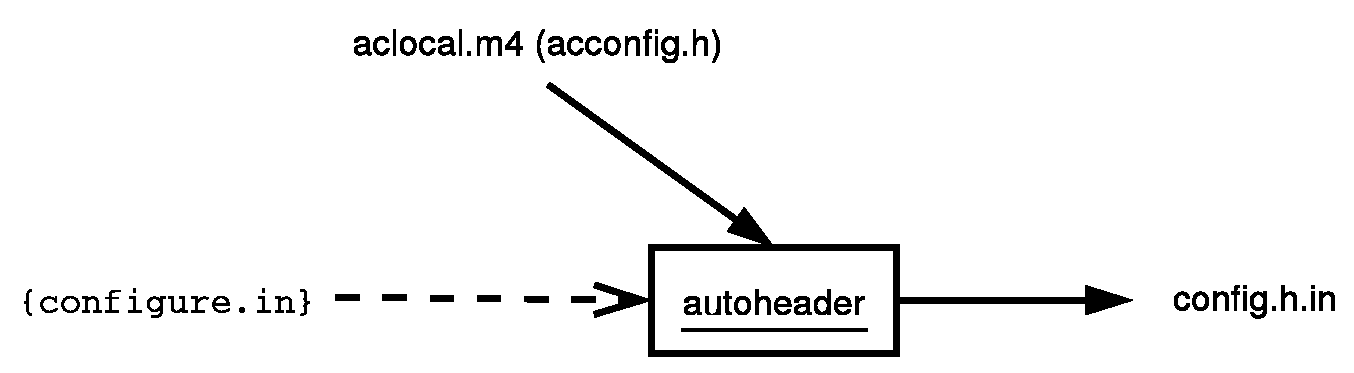
\includegraphics[scale=.35]{fig/DiagrammeAutoheader}
\end{center}

\subsection{Automake and Libtoolize}
Automake\footnote{Automake {\url{http://www.gnu.org/software/automake/automake.html}}} 
will call libtoolize to generate some extra files if the macro 
'AC\_PROG\_LIBTOOL' is used in `configure.in'. If it is not present 
then automake will install `config.guess' and `config.sub' by itself.

libtoolize\footnote{Libtool {\url{http://www.gnu.org/software/libtool/libtool.html}}}
can also be run manually if desired. 
Automake will only run libtoolize automatically if `ltmain.sh' and `ltconfig' 
are missing. In DIET, we choose to call explicitly libtoolize before automake
in bootstrap.sh.

\begin{center}
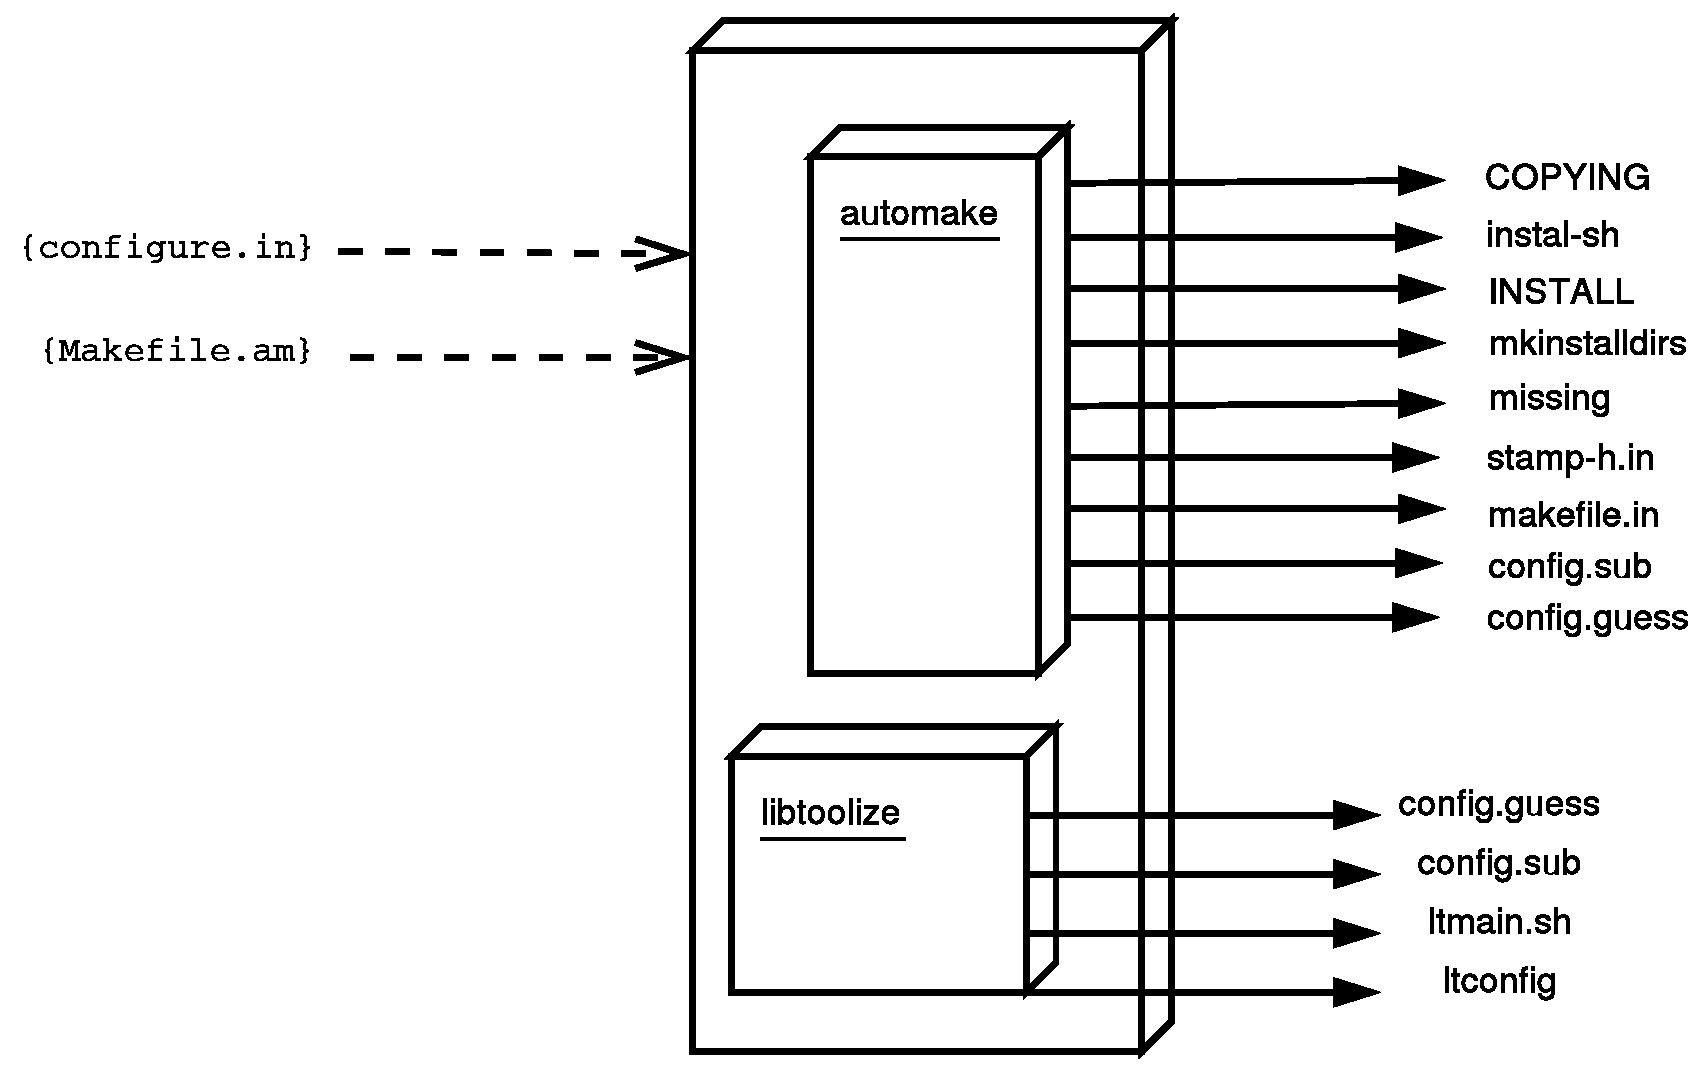
\includegraphics[scale=.35]{fig/DiagrammeAutomakeLibtoolize}
\end{center}

The versions of `config.guess' and `config.sub' installed differ between 
releases of Automake and Libtool, and might be different depending on whether 
libtoolize is used to install them or not. Before releasing your own package 
you should get the latest versions of these files from ftp://ftp.gnu.org/gnu/config,
in case there have been changes since releases of the GNU Autotools.
Currently, DIET is developped with, at least, libtool 1.4.3, automake 1.7.3 and 
autoconf 2.57. Bootstraping and compiling may succeed with others previous autotools version
but it is not garanteed.
%\footnote{Automake {\url{http://www.gnu.org/software/automake/automake.html}}}
%\footnote{Libtool {\url{http://www.gnu.org/software/libtool/libtool.html}}}


\subsection{autoconf}
autoconf\footnote{Autoconf {\url{http://www.gnu.org/software/autoconf/}}} expands the m4 macros in `configure.in', using macro 
definitions from `aclocal.m4', to generate the configure script.
\begin{center}
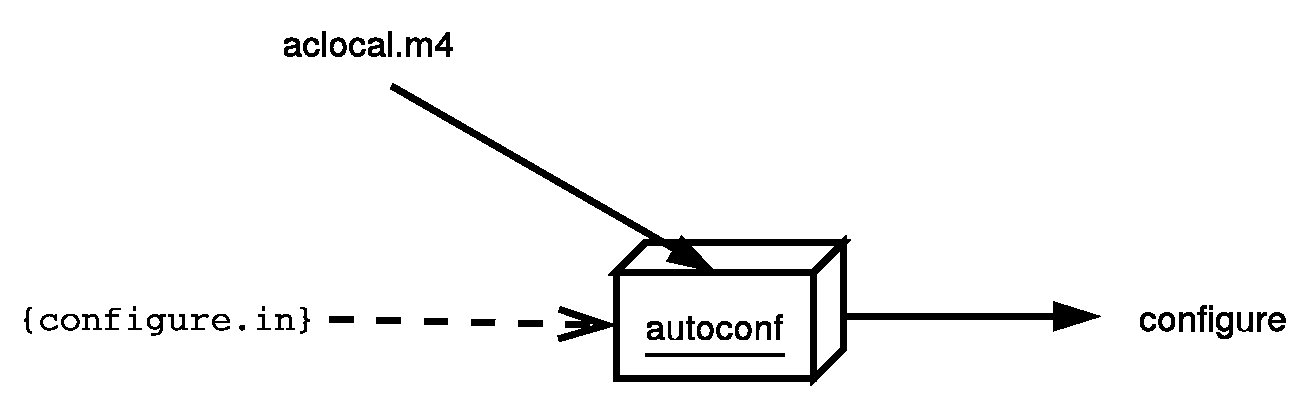
\includegraphics[scale=.35]{fig/DiagrammeAutoconf}
\end{center}
%\footnote{Autoconf {\url{http://www.gnu.org/software/autoconf/}}}

\subsection{configure}
The purpose of the preceding processes was to create the input files necessary
for configure to run correctly. You would ship your project with the generated
script and the files in columns, other input and processes (except 
`config.cache'), but configure is designed to be run by the person installing
your package. Naturally, you will run it too while you develop your project,
but the files it produces are specific to your development machine, and are
not shipped with your package -- the person installing it later will run 
configure and generate output files specific to their own machine.

Running the configure script on the build host executes the various tests 
originally specified by the `configure.in' file, and then creates another script,
`config.status'. This new script generates the `DIET\_config.h' header file from 
`DIET\_config.h.in', and `Makefile's from the named `Makefile.in's. Once 
`config.status' has been created, it can be executed by itself to regenerate
files without rerunning all the tests. Additionally, `AC\_PROG\_LIBTOOL'
was used, so ltconfig is used to generate a libtool script. 

\begin{center}
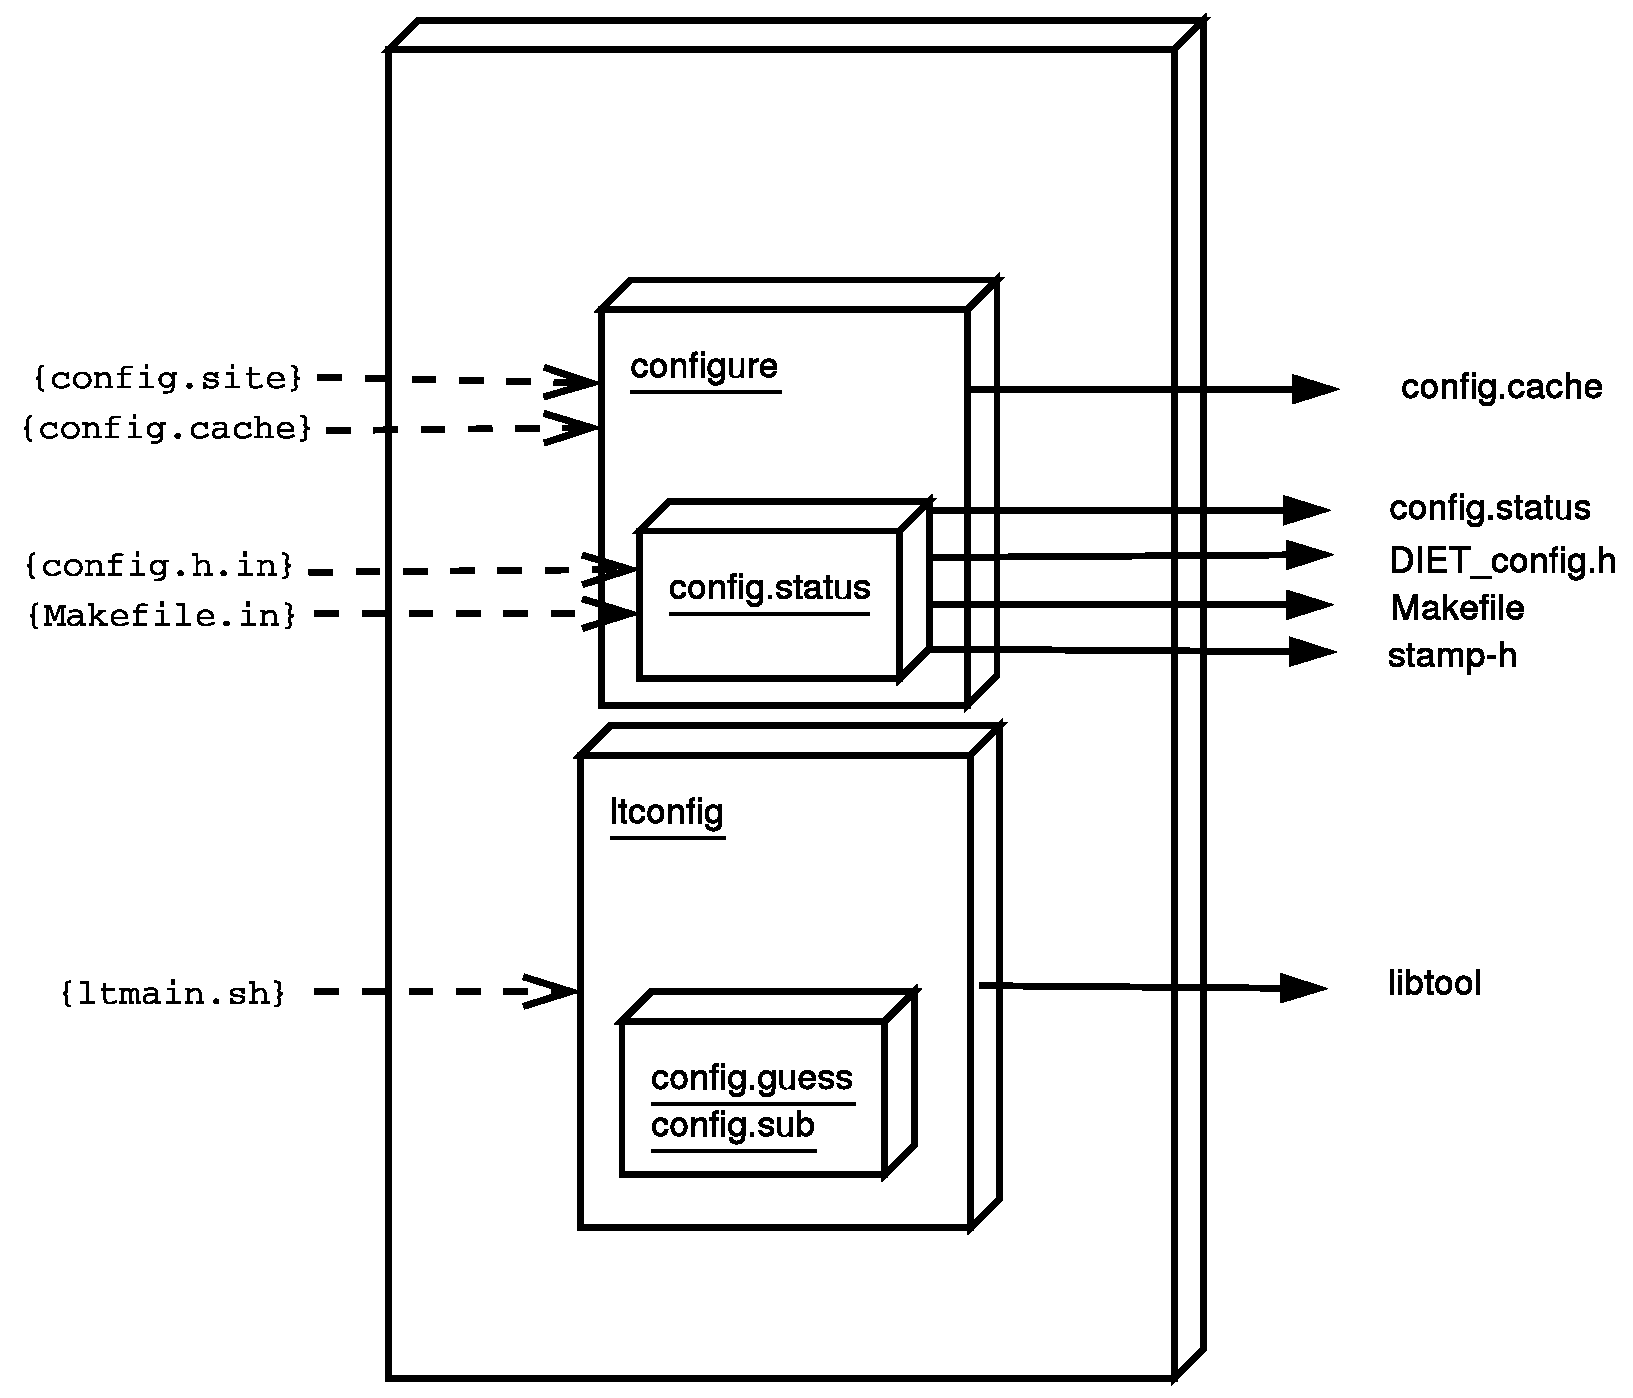
\includegraphics[scale=.35]{fig/DiagrammeConfigure}
\end{center}

\section{CORBA and asynchronism}
Datas from the book "Advanced CORBA Programming with C++""
\footnote{"Advanced CORBA Programming with C++"  from Michi Henning, Steve Vinoski} and
from omniORB\footnote{OMNIORB {\url{http://www.uk.research.att.com/omniORB/}}}
and from TAO\footnote{TAO {\url{http://www.cs.wustl.edu/~schmidt/TAO.html}}
}



%%%%
% Reference 
%%%%


\
\end{document}

